\section{Resoconto delle Attività di Verifica}\label{Resoconto}
\subsection{Scopo}

In questa sezione, vengono mostrati i risultati derivanti dalla misurazione delle metriche utilizzate.

\subsection{Revisione dei Requisiti}


\subsubsection{Metriche}

\begin{longtable}{|C{.16\textwidth}|C{.16\textwidth}|C{.36\textwidth}|C{.20\textwidth}|}
\hline
\rowcolor{bluelogo}\textbf{\textcolor{white}{Processo}} & \textbf{\textcolor{white}{Risultato}} & \textbf{\textcolor{white}{Descrizione}} & \textbf{\textcolor{white}{Valutazione}}\\
PR01 \{MTPC01\} & +0 & Il gruppo è riuscito a svolgere le attività entro le date prestabilite. & Ottimo \\
\hline

\rowcolor{grigio}PR02 \{MTPC02\} & \EUR{+135.00} \{+3.37\%\} & Sono state necessarie più ore all'inizio. & Accettabile\\
\hline

PR02 \{MTPC03\} & \EUR{+135.00} \{+0.74\%\} & Sono state necessarie più ore all'inizio. & Accettabile\\
\hline

\rowcolor{grigio}PR04 \{MTPC09\} & +0 & Non si sono manifestati nuovi rischi. & Ottimo\\
\hline

\caption{Risultati Misurazioni: Avvio ed Analisi dei Requisiti}
\label{ris:aar}
\end{longtable}

\subsubsection{Maturità dei Processi}

\begin{longtable}{|C{.47\textwidth}|C{.47\textwidth}|}
\hline
\rowcolor{bluelogo}\textbf{\textcolor{white}{Processo}} & \textbf{\textcolor{white}{Maturità}}\\
PR01 & 2\\ 
\hline
\rowcolor{grigio}PR02 & 2 \\
\hline
PR04 & 1 \\ 
\hline 
\caption{Maturità Processi: Avvio ed Analisi dei Requisiti}
\label{mat:aar}
\end{longtable}


\subsubsection{Indice di Gulpease}


\begin{longtable}{|C{.47\textwidth}|C{.22\textwidth}|C{.22\textwidth}|}
\hline
\rowcolor{bluelogo}\textbf{\textcolor{white}{Documento}} & \textbf{\textcolor{white}{Risultato}} & \textbf{\textcolor{white}{Valutazione}}\\
\endhead
\textit{Norme di Progetto v1.0.0} & 55.16 & Accettabile \\
\hline
\rowcolor{grigio}\textit{Studio di Fattibilità v1.0.0} & 50.58 & Accettabile\\
\hline
\textit{Analisi dei Requisiti v1.0.0} & 53.65 & Accettabile \\
\hline
\rowcolor{grigio}\textit{Glossario v1.0.0} & 48.50 & Accettabile\\
\hline
\textit{Piano di Progetto v1.0.0} & 47.21 & Accettabile \\
\hline
\rowcolor{grigio}\textit{Piano di Qualifica v1.0.0} & 48.83 & Accettabile\\

\hline
\textit{Verbale Interno 2018-11-21} & 53.10 & Accettabile\\
\hline
\rowcolor{grigio}\textit{Verbale Interno 2018-11-28} & 57.06 & Accettabile\\
\hline
\textit{Verbale Interno 2018-12-13} & 55.82 & Accettabile\\
\hline
\rowcolor{grigio}\textit{Verbale Interno 2018-12-20} & 56.47 & Accettabile \\
\hline
\textit{Verbale Interno 2019-01-02} & 54.42 & Accettabile \\
\hline
\rowcolor{grigio}\textit{Verbale Interno 2019-01-10} & 62.25 & Accettabile\\
\hline
\textit{Verbale Esterno 2018-12-10} & 55.28 & Accettabile\\
\hline
\rowcolor{grigio}\textit{Lettera di Presentazione} & 64.09 & Accettabile\\
\hline
\textit{Corrispondenza 2018-12-06} & 47.42 & Accettabile\\
\hline

\caption{Indice di Gulpease: Avvio ed Analisi dei Requisiti}
\label{gulp:aar}
\end{longtable}


\newpage

\subsection{Revisione di Progettazione}\label{RevisioneP}
\subsubsection{Metriche}

\paragraph{Maturità dei Processi} \-\\

\begin{figure}[H]
	\begin{center}
		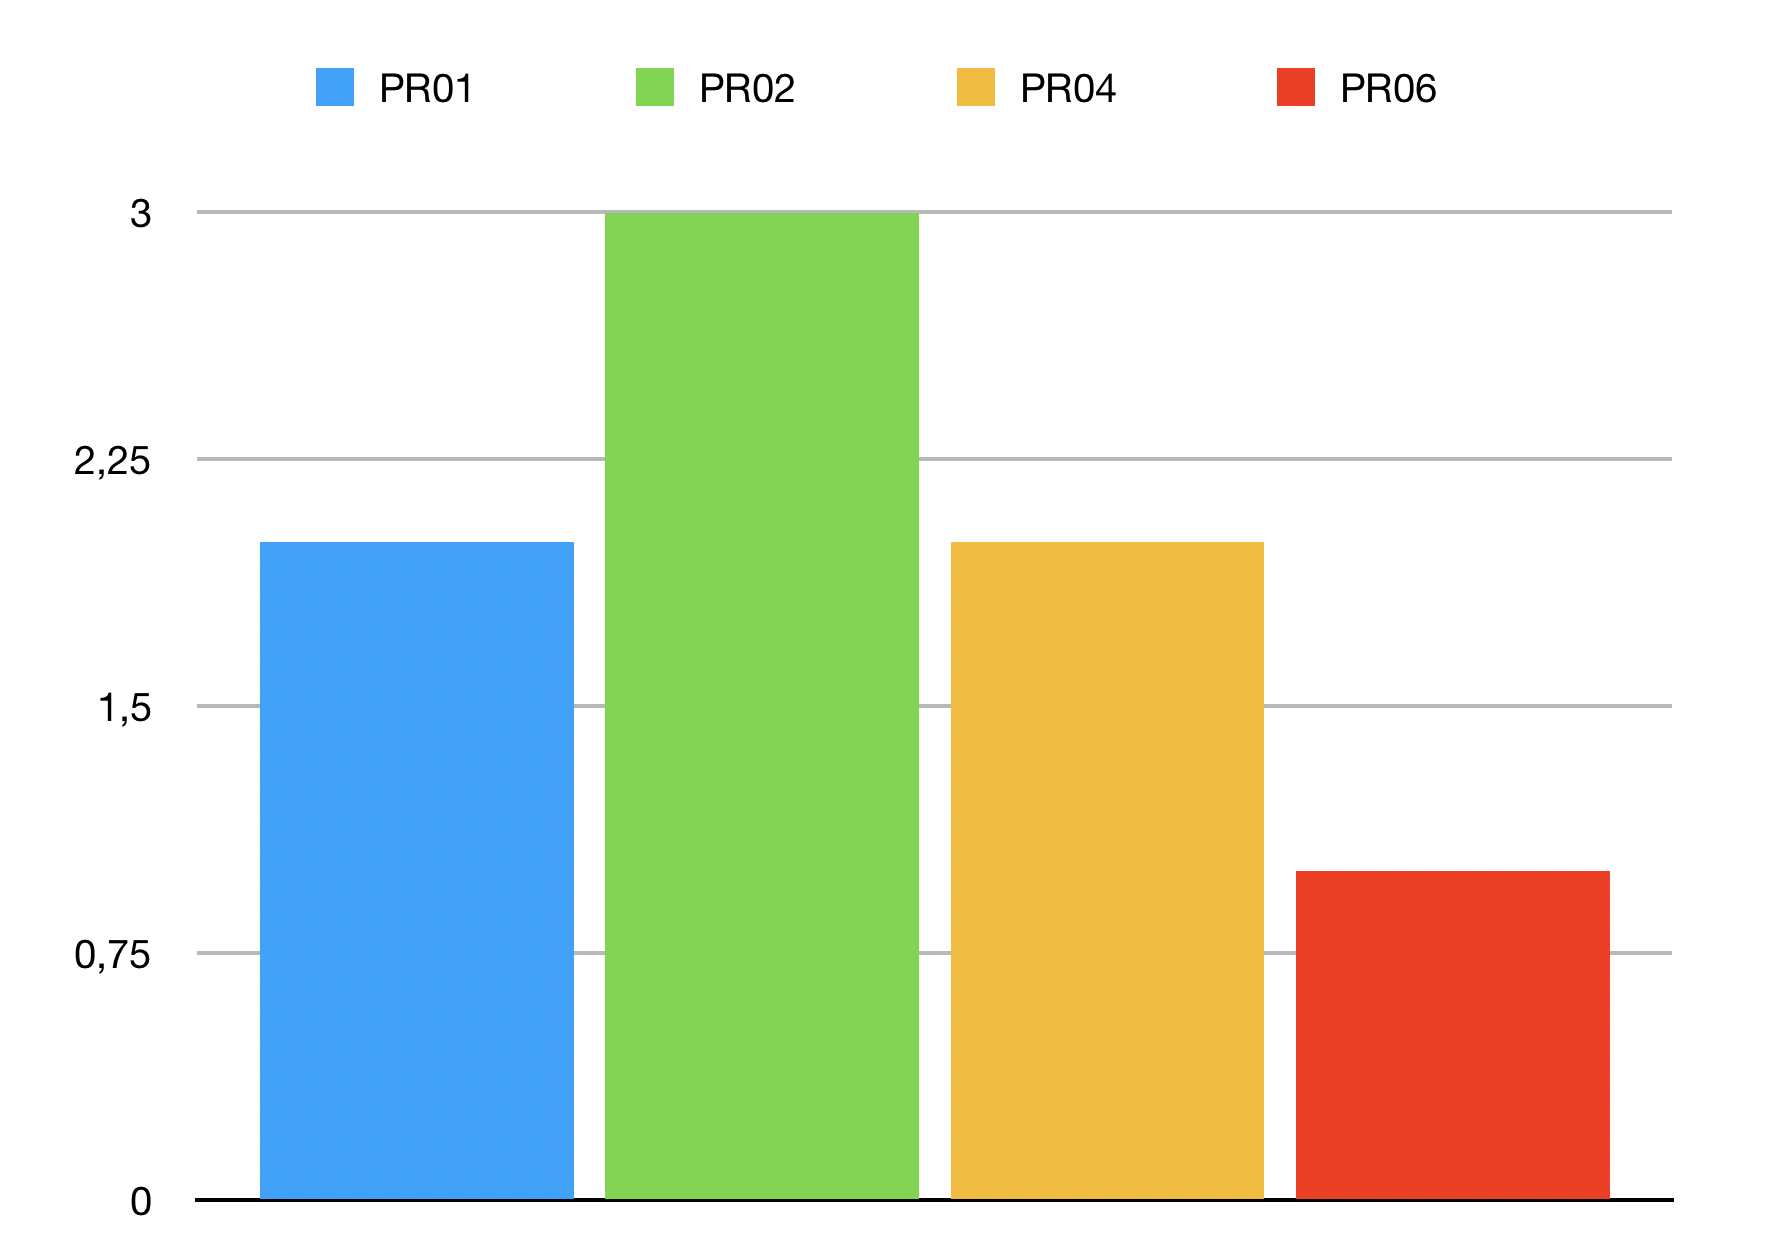
\includegraphics[scale=0.4]{./images/grafici_RP/CMMI.png} 
	\end{center}
	\caption{RP : CMMI}
\end{figure}

\pagebreak

\paragraph{MTPC01: Schedule Variance} ~\\
\begin{figure}[H]
	\begin{center}
		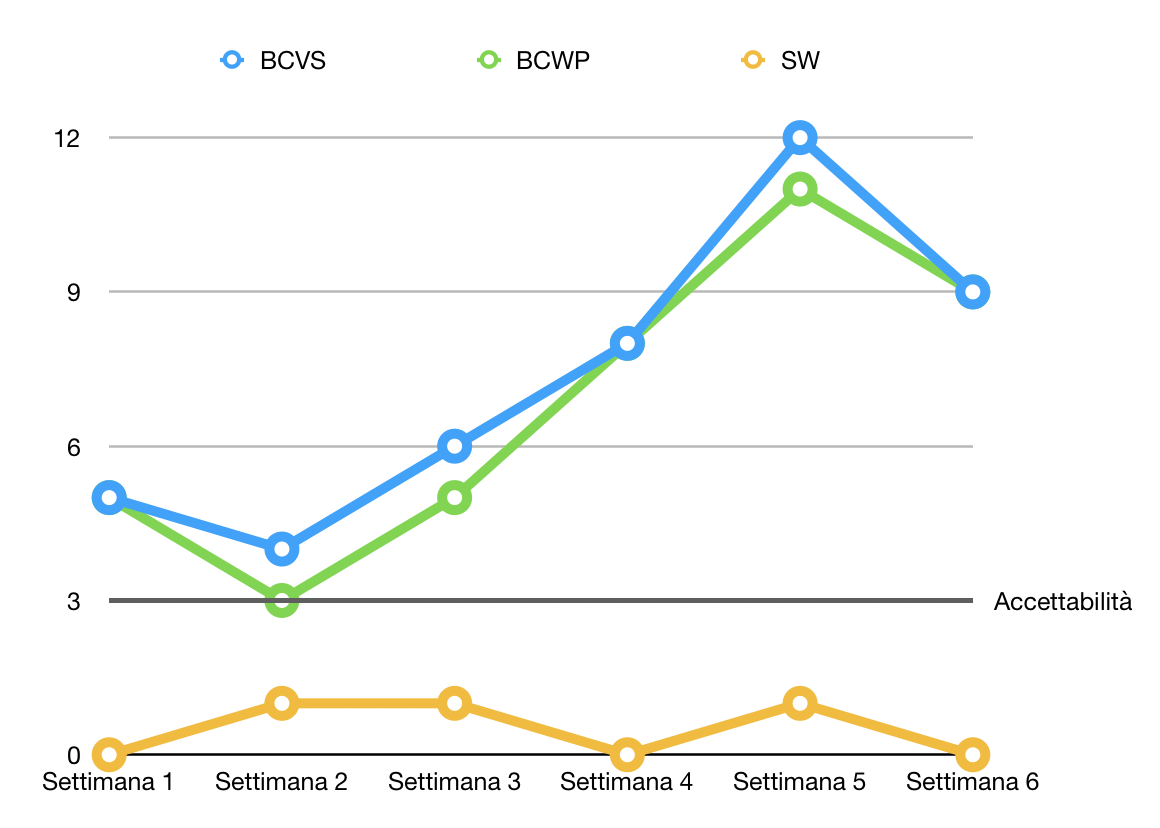
\includegraphics[scale=0.5]{./images/grafici_RP/MTPC01.png} 
	\end{center}
	\caption{RP : MTPC01}
\end{figure}

\paragraph{MTPC02: Budget Variance}\-\\
\begin{figure}[H]
	\begin{center}
		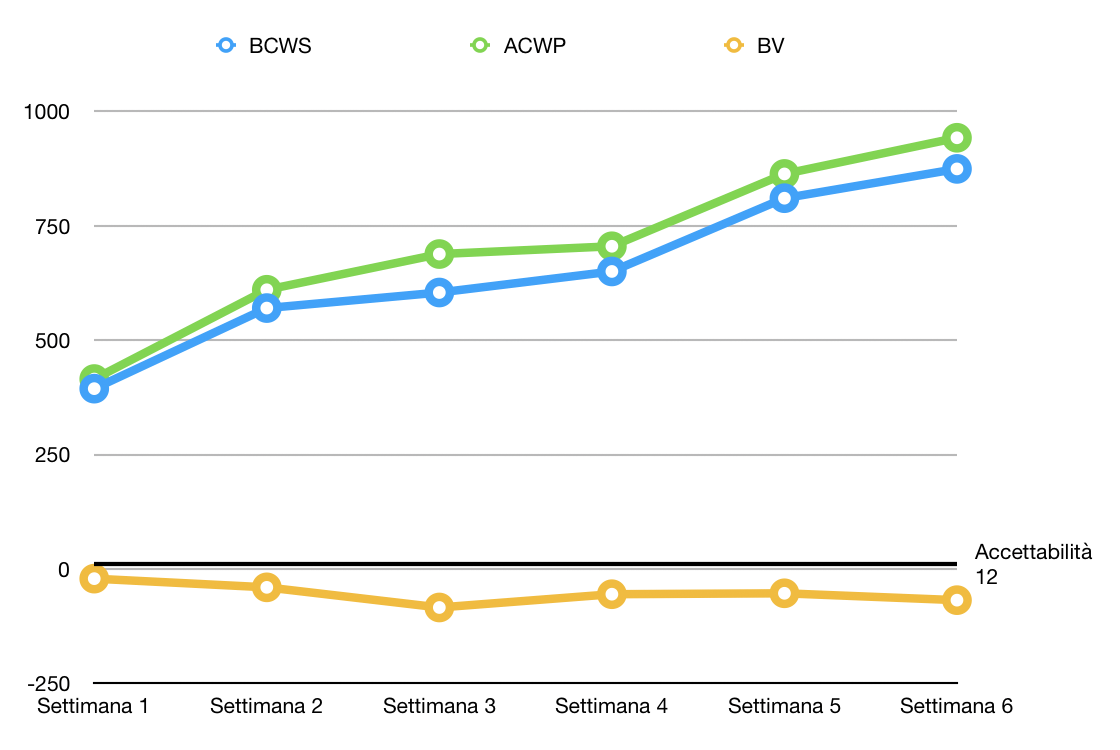
\includegraphics[scale=0.5]{./images/grafici_RP/MTPC02.png} 
	\end{center}
	\caption{RP : MTPC02}
\end{figure}

\pagebreak

\paragraph{MTPC03: Estimated at Completion}\-\\
\begin{figure}[H]
	\begin{center}
		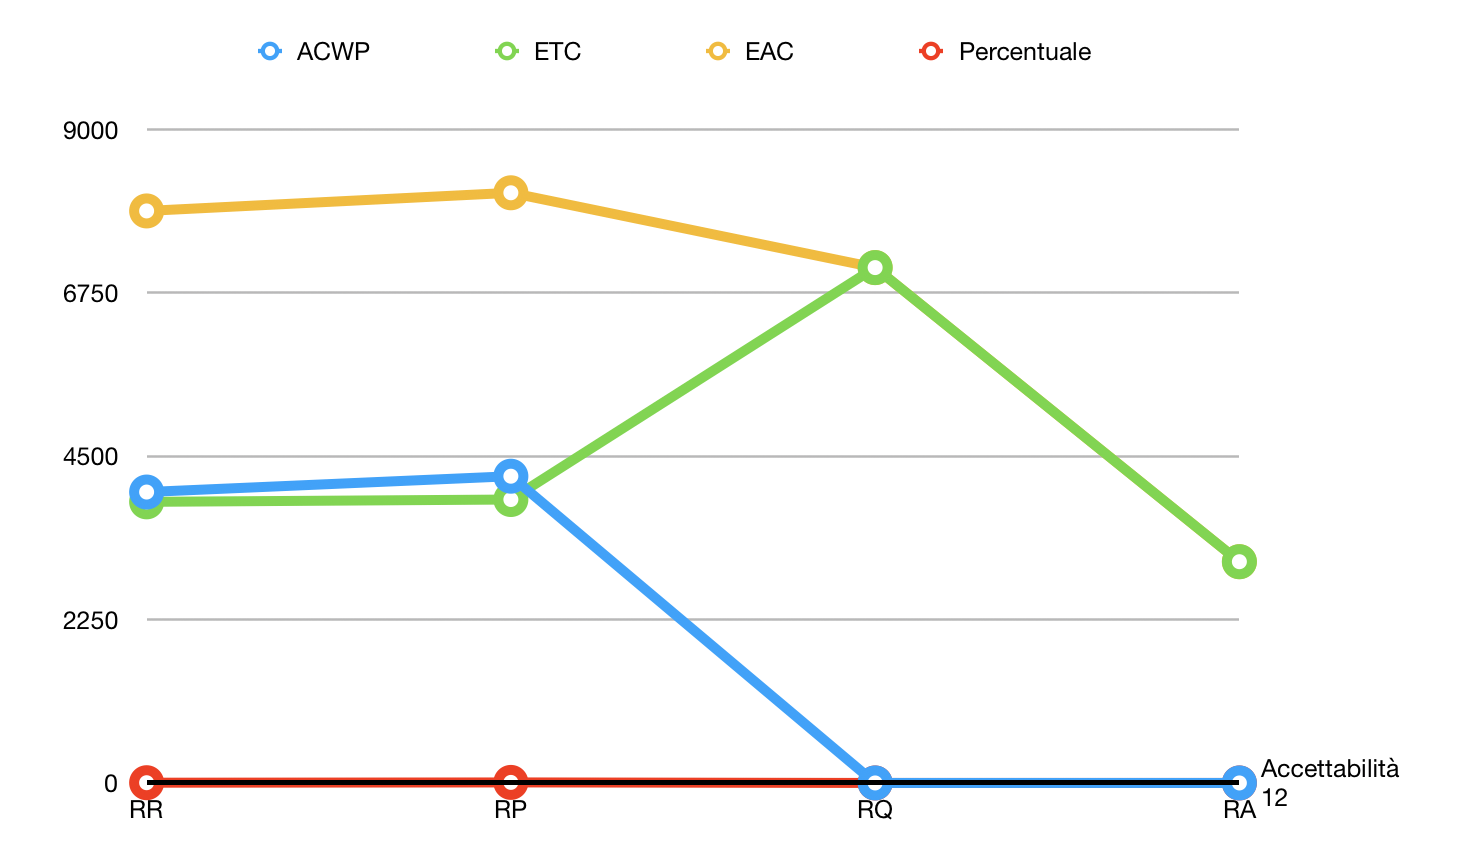
\includegraphics[scale=0.5]{./images/grafici_RP/MTPC03.png} 
	\end{center}
	\caption{RP : MTPC03}
\end{figure}

\paragraph{MTPC16: Media Commit per Settimana}\-\\
\begin{figure}[H]
	\begin{center}
		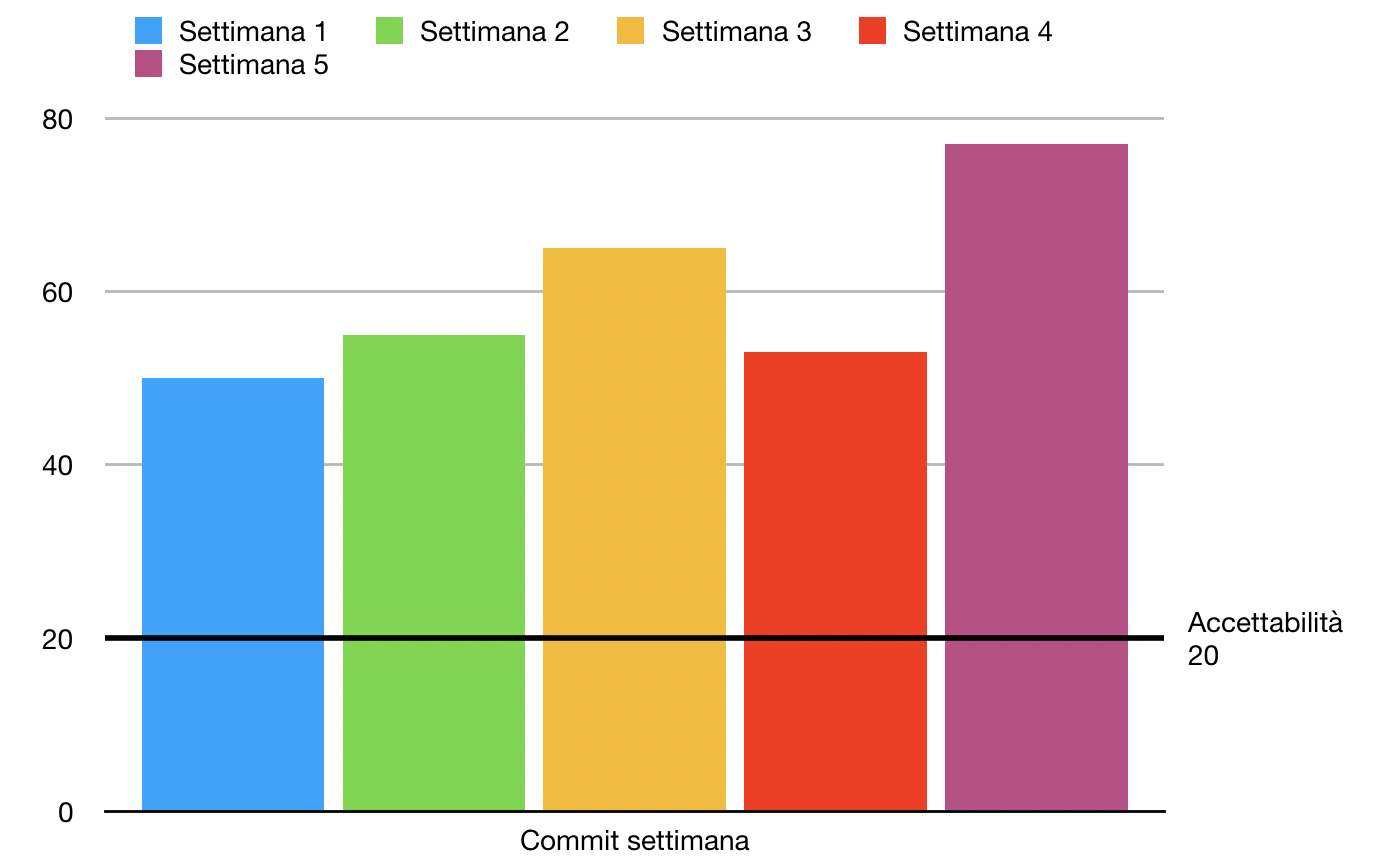
\includegraphics[scale=0.5]{./images/grafici_RP/commitGithub.png} 
	\end{center}
	\caption{RP : MTPC17 - GitHub}
\end{figure}

\begin{figure}[H]
	\begin{center}
		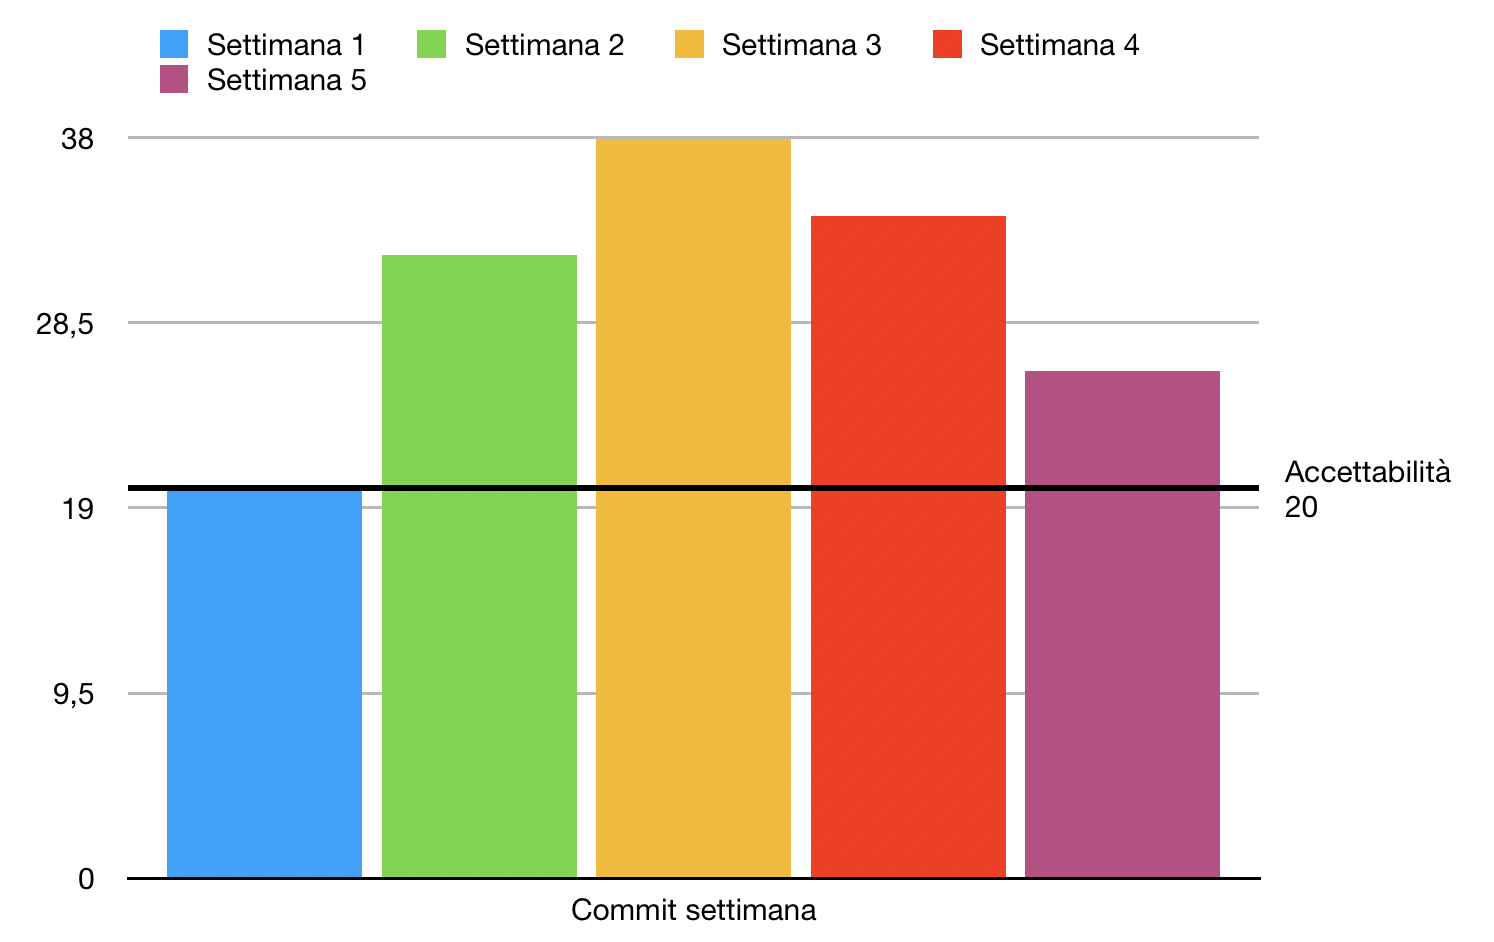
\includegraphics[scale=0.5]{./images/grafici_RP/commitGitlab.png} 
	\end{center}
	\caption{RP : MTPC17 - GitLab}
\end{figure}


\paragraph{MTPC18: Percentuali Build Superate}\-\\

\begin{longtable}{|C{.15\textwidth}|C{.24\textwidth}|C{.24\textwidth}|}
\hline
\rowcolor{bluelogo}\textbf{\textcolor{white}{Ottimalità}} & \textbf{\textcolor{white}{Accettabilità}} & \textbf{\textcolor{white}{Valore Misurato}} \\
\hline \hline
\endhead
 $\geq 80$\% & $\geq 65$\% & 68.1\% \\
\hline

\caption{MTPC18 - Percentuale Build Superate}
\label{mtpc17}
\end{longtable}
\begin{figure}[H]
	\begin{center}
		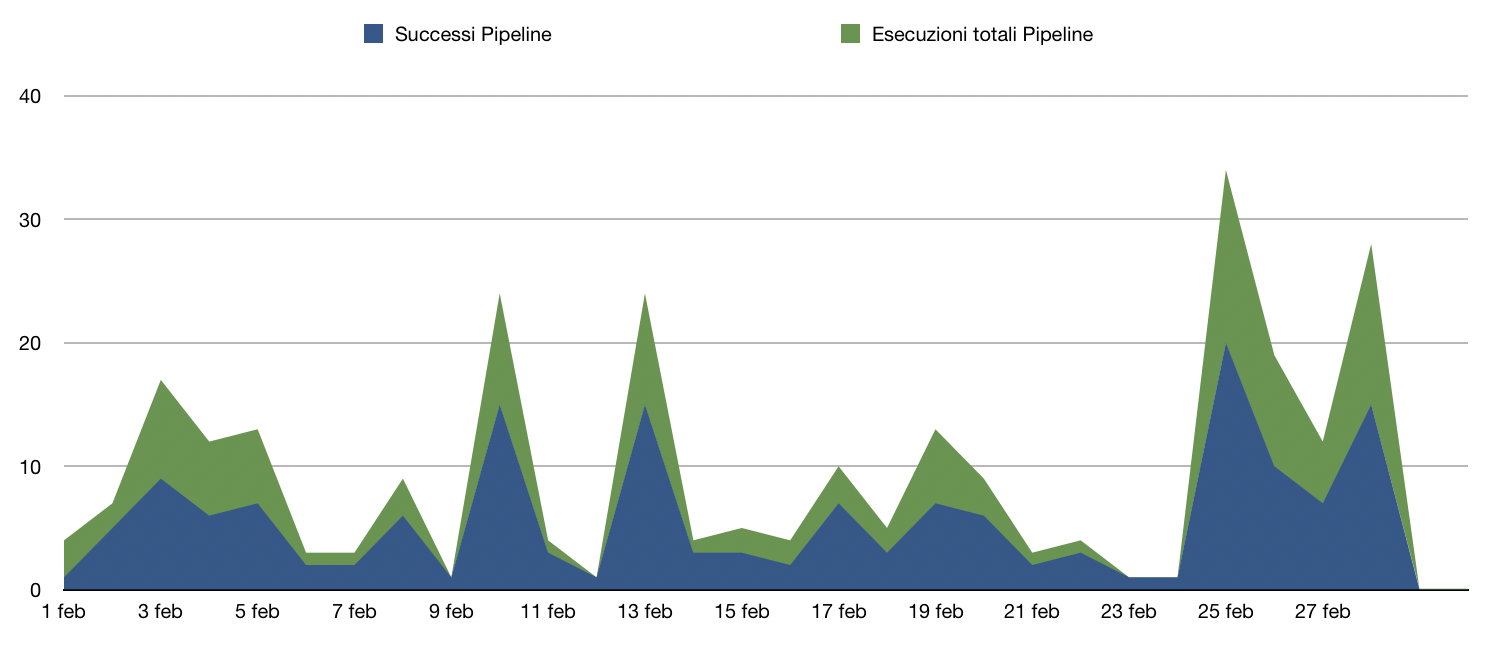
\includegraphics[scale=0.5]{./images/grafici_RP/graficoPipeline.png} 
	\end{center}
	\caption{RP : MTPC18}
\end{figure}

\pagebreak

\paragraph{MTPDD19: Indice di Gulpease}\-\\
\label{gulpi}

\begin{figure}[H]
	\begin{center}
		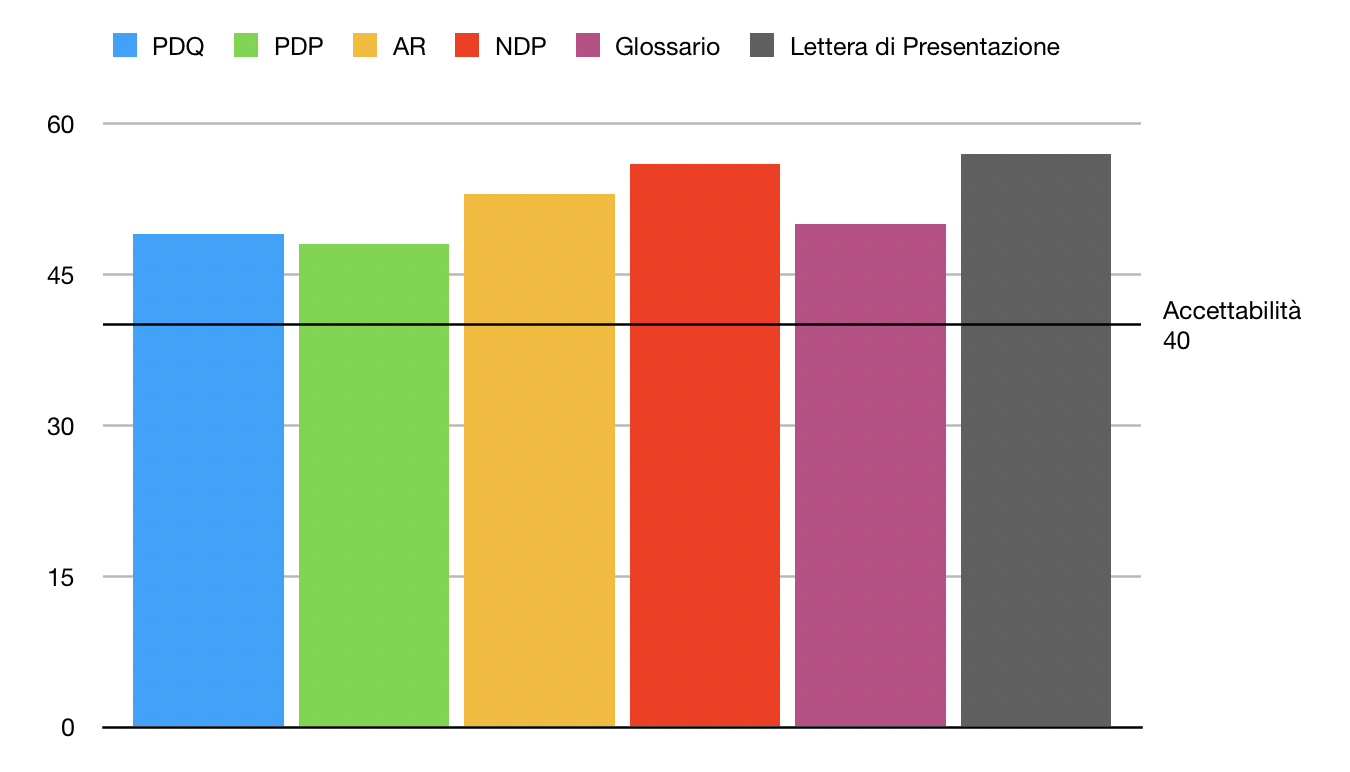
\includegraphics[scale=0.6]{./images/grafici_RP/gulpeasedocumenti.png} 
	\end{center}
	\caption{RP : MTPDD19 - Documentazione}
\end{figure}

\begin{figure}[H]
	\begin{center}
		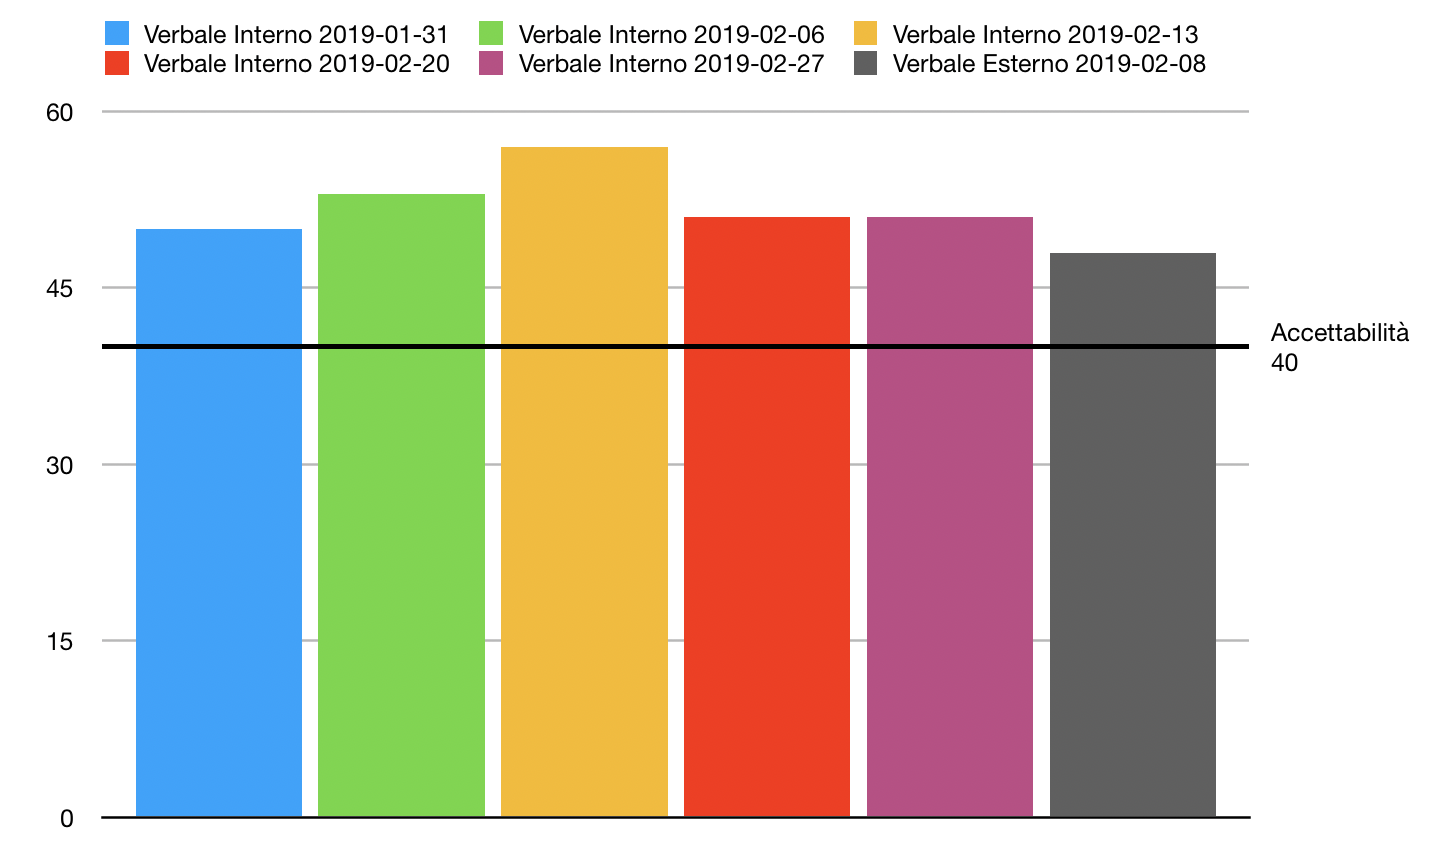
\includegraphics[scale=0.5]{./images/grafici_RP/gulpeaseverbali.png} 
	\end{center}
	\caption{RP : MTPDD19 - Verbali Interni ed Esterni}
\end{figure}


\newpage
\subsection{Revisione di Qualifica}\label{metricheRQ}
\subsubsection{Metriche}
\paragraph{Maturità dei Processi}
\begin{figure}[H]
	\begin{center}
		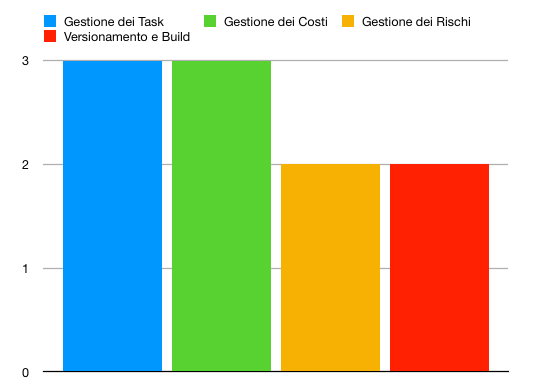
\includegraphics[scale=0.5]{./images/grafici_RQ/maturitaProcessi.png} 
	\end{center}
	\caption{RQ: CMMI}
\end{figure}


\paragraph{MTPC01: Schedule Variance} ~\\
\begin{figure}[H]
	\begin{center}
		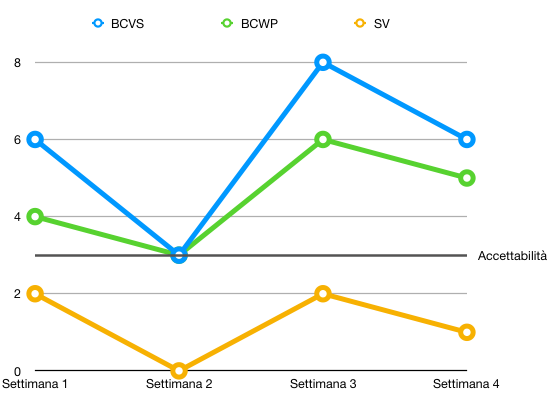
\includegraphics[scale=0.5]{./images/grafici_RQ/MTPC01.png} 
	\end{center}
	\caption{RQ : MTPC01}
\end{figure}

\paragraph{MTPC02: Budget Variance}\-\\
\begin{figure}[H]
	\begin{center}
		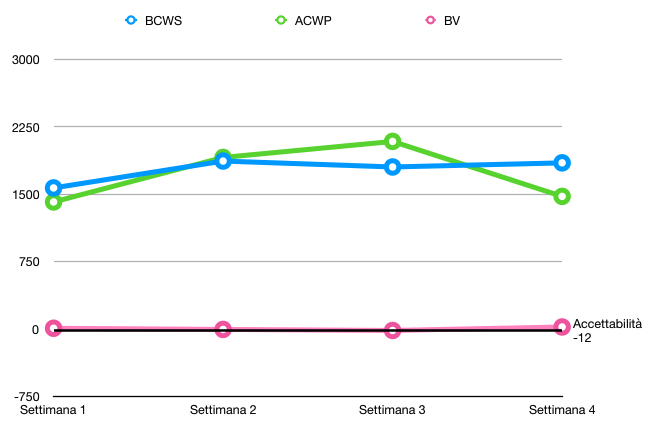
\includegraphics[scale=0.5]{./images/grafici_RQ/MTPC02.png} 
	\end{center}
	\caption{RQ : MTPC02}
\end{figure}

\pagebreak

\paragraph{MTPC03: Estimated at Completion}\-\\
\begin{figure}[H]
	\begin{center}
		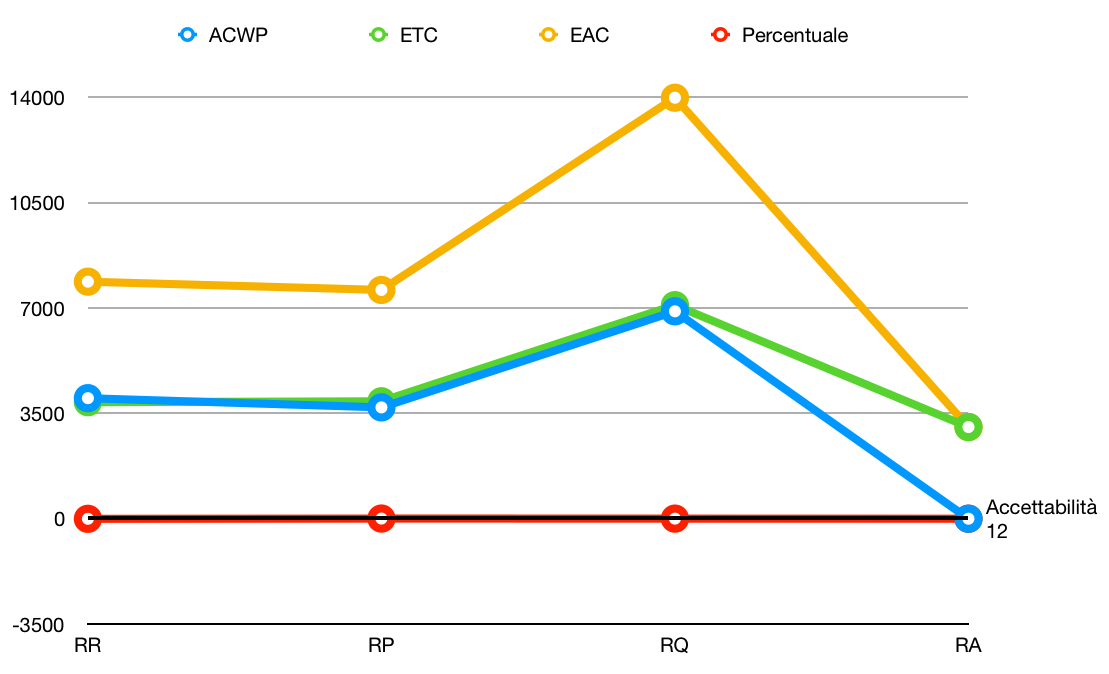
\includegraphics[scale=0.3]{./images/grafici_RQ/MTPC03.png} 
	\end{center}
	\caption{RQ : MTPC03}
\end{figure}

\pagebreak

\paragraph{MTPC08: Code Coverage} \-\\
\begin{figure}[H]
	\begin{center}
		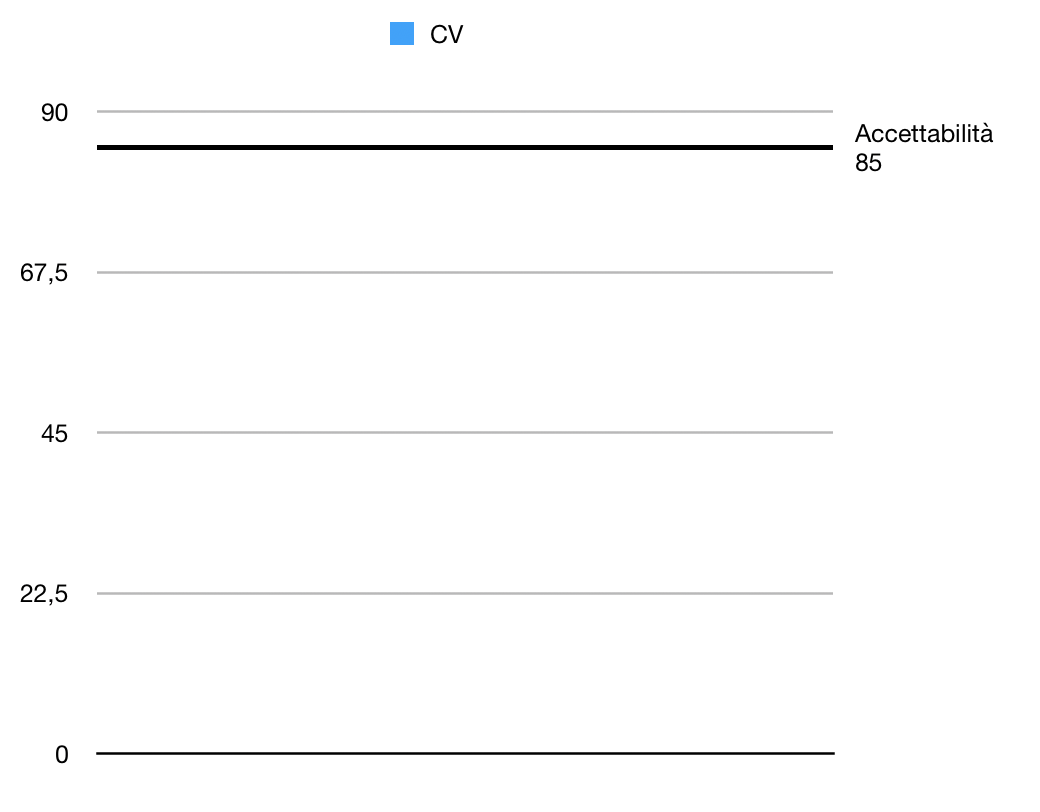
\includegraphics[scale=0.5]{./images/grafici_RQ/MTPC08.png}
	\end{center}
	\caption{RQ: MTPC08}
\end{figure}

\paragraph{MTPC17: Media Commit per Settimana}\-\\
\begin{figure}[H]
	\begin{center}
		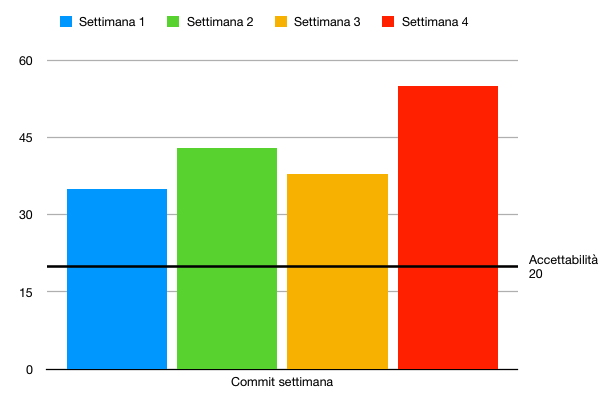
\includegraphics[scale=0.5]{./images/grafici_RQ/commitSettimana.png} 
	\end{center}
	\caption{RQ : MTPC17}
\end{figure}

\pagebreak

\paragraph{MTPC18: Percentuali Build Superate}\-\\

\begin{longtable}{|C{.15\textwidth}|C{.24\textwidth}|C{.24\textwidth}|}
	\hline
	\rowcolor{bluelogo}\textbf{\textcolor{white}{Ottimalità}} & \textbf{\textcolor{white}{Accettabilità}} & \textbf{\textcolor{white}{Valore Misurato}} \\
	\hline \hline
	\endfirsthead
	$\geq 80$\% & $\geq 65$\% & 71.8\% \\
	\hline
	\caption{MTPC18 - Percentuale Build Superate}
	\label{mtpc17}
\end{longtable}
\begin{figure}[H]
	\begin{center}
		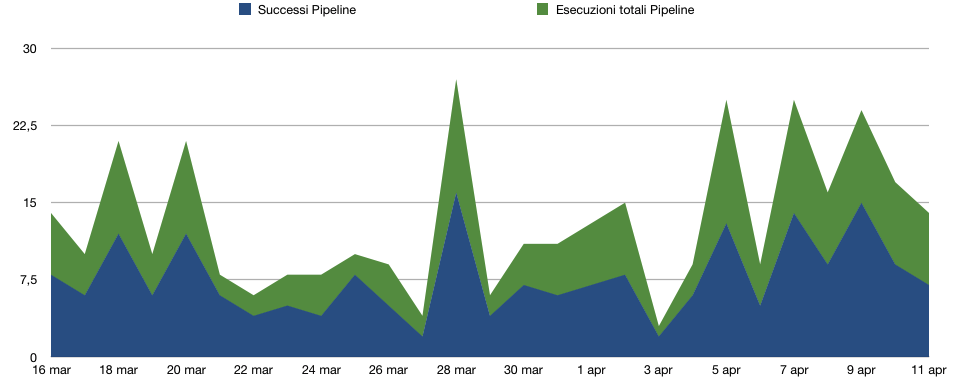
\includegraphics[scale=0.5]{./images/grafici_RQ/pipeline.png} 
	\end{center}
	\caption{RQ : MTPC18}
\end{figure}

\pagebreak

\paragraph{MTPDD19: Indice di Gulpease}\-\\
\label{gulpiRQ}

\begin{figure}[H]
	\begin{center}
		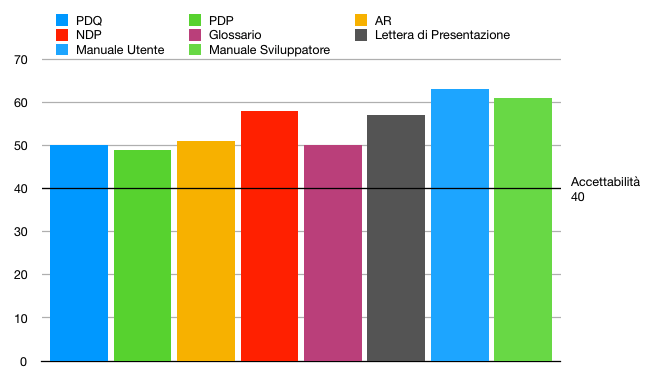
\includegraphics[scale=0.6]{./images/grafici_RQ/gulpeaseDocumenti.png} 
	\end{center}
	\caption{RQ: MTPDD19 - Documentazione}
\end{figure}

\begin{figure}[H]
	\begin{center}
		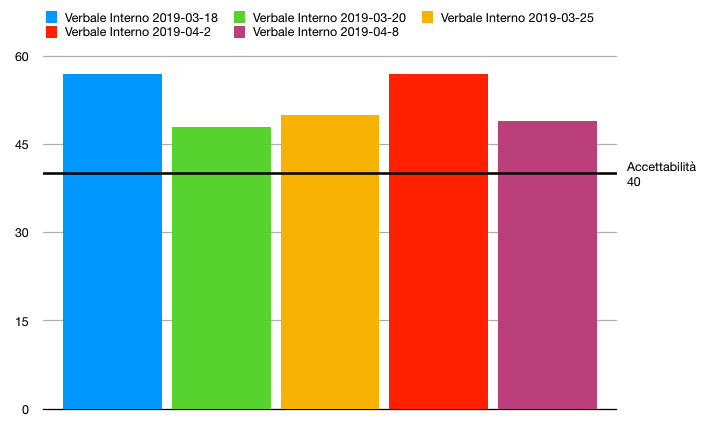
\includegraphics[scale=0.5]{./images/grafici_RQ/gulpeaseVerbali.png} 
	\end{center}
	\caption{RQ: MTPDD19 - Verbali Interni}
\end{figure}

\pagebreak

\paragraph{MTPDS21 - MTPDS22 - MTPDS23: Copertura Requisiti}\-\\\label{copReq}

\begin{minipage}[t]{0.25\textwidth}
	\begin{figure}[H]
		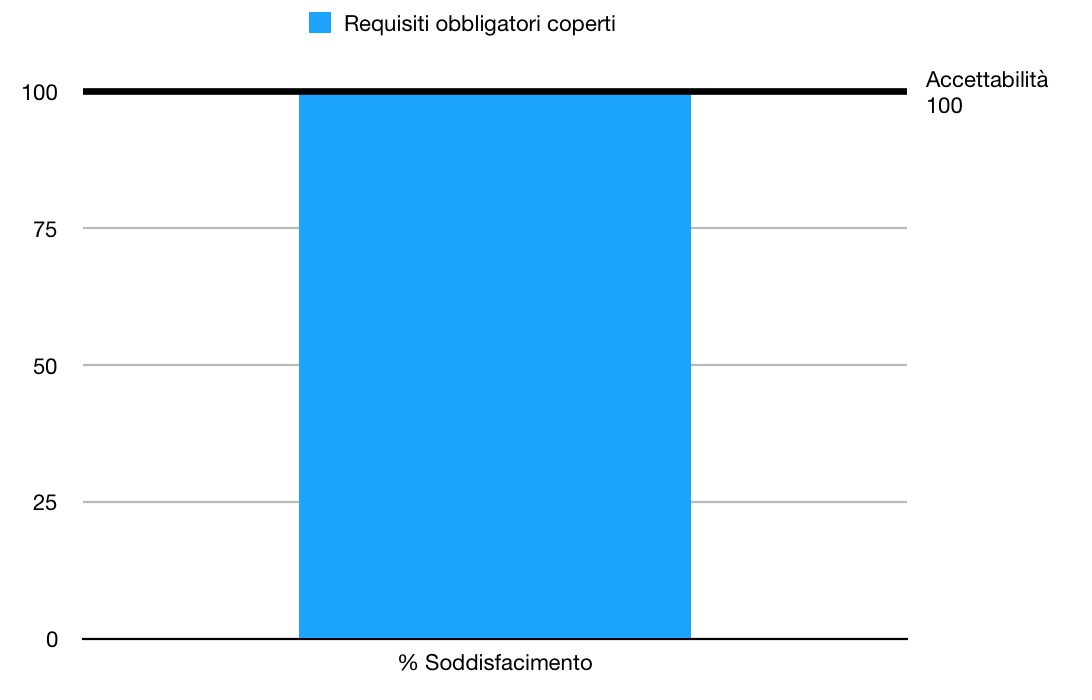
\includegraphics[scale=0.3]{./images/grafici_RQ/reqObbCop.png} 
		\caption{\-\\Requisiti obbligatori coperti}
	\end{figure}
\end{minipage}
\begin{minipage}[t]{0.25\textwidth}
	\begin{figure}[H]
		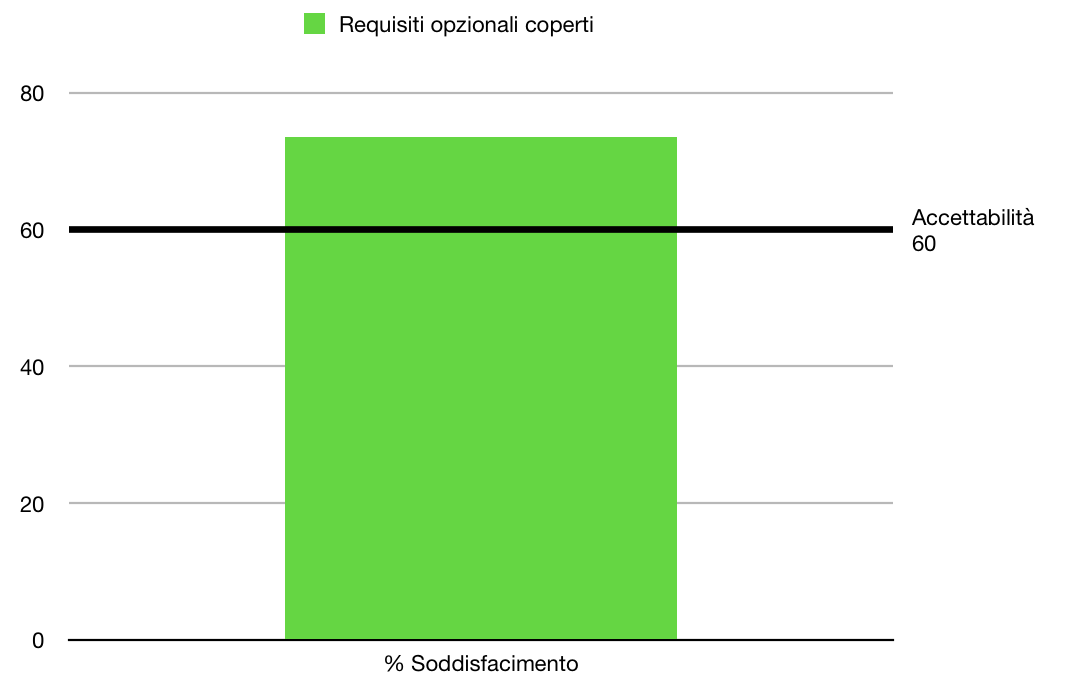
\includegraphics[scale=0.3]{./images/grafici_RQ/reqOpzCop.png} 
		\caption{\-\\Requisiti opzionali coperti}
	\end{figure}
\end{minipage}
\begin{minipage}[t]{0.25\textwidth}
	\begin{figure}[H]
		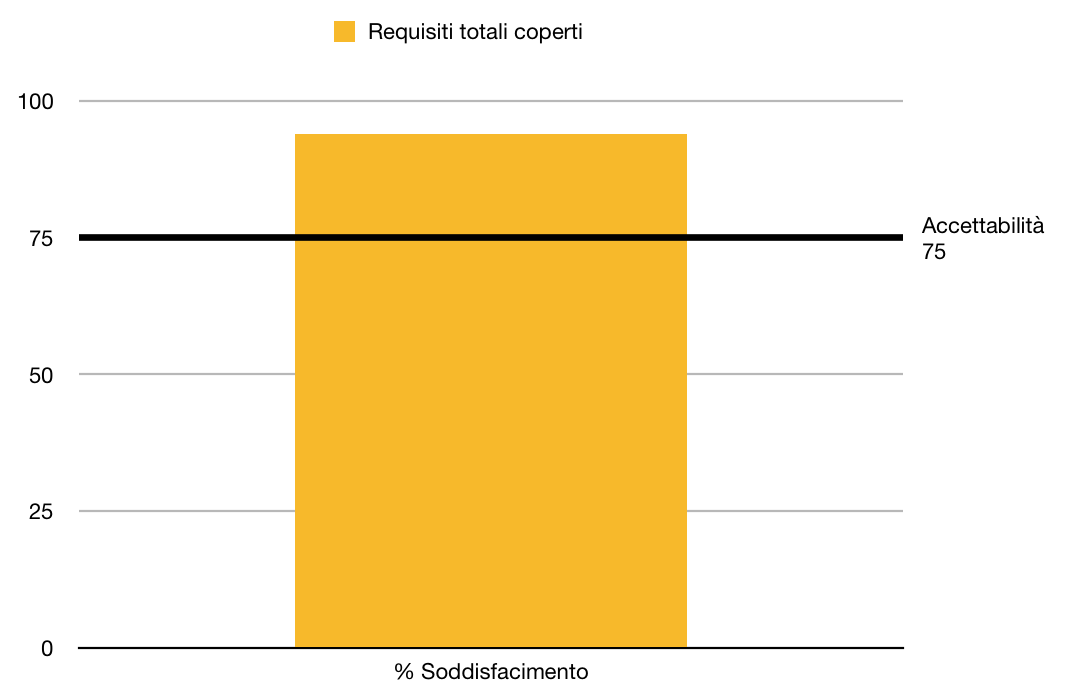
\includegraphics[scale=0.3]{./images/grafici_RQ/reqTotCop.png} 
		\caption{\-\\Requisiti totali coperti}
	\end{figure}
\end{minipage}

\pagebreak

\subsection{Revisione di Accettazione}
\label{RA_metriche}

\subsubsection{Maturità dei Processi} 
\begin{figure}[H]
	\begin{center}
	
		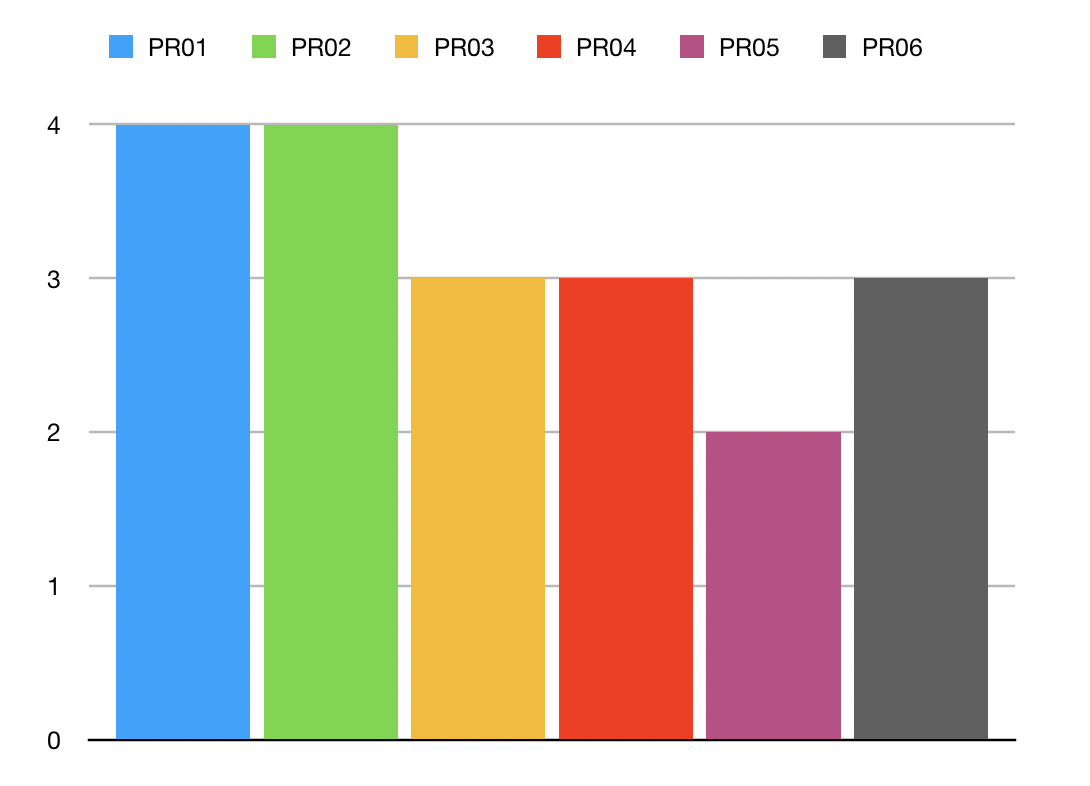
\includegraphics[scale=0.5]{./images/grafici_RA/CMMI.png} 
		\caption{RA: CMMI}
		
	\end{center}
	\end{figure}

\subsubsection{Metriche}

\paragraph{PR01: Gestione dei Task}
\subparagraph{MTPC01: Schedule Variance}  \-\\

\begin{figure}[H]
	\begin{center}
		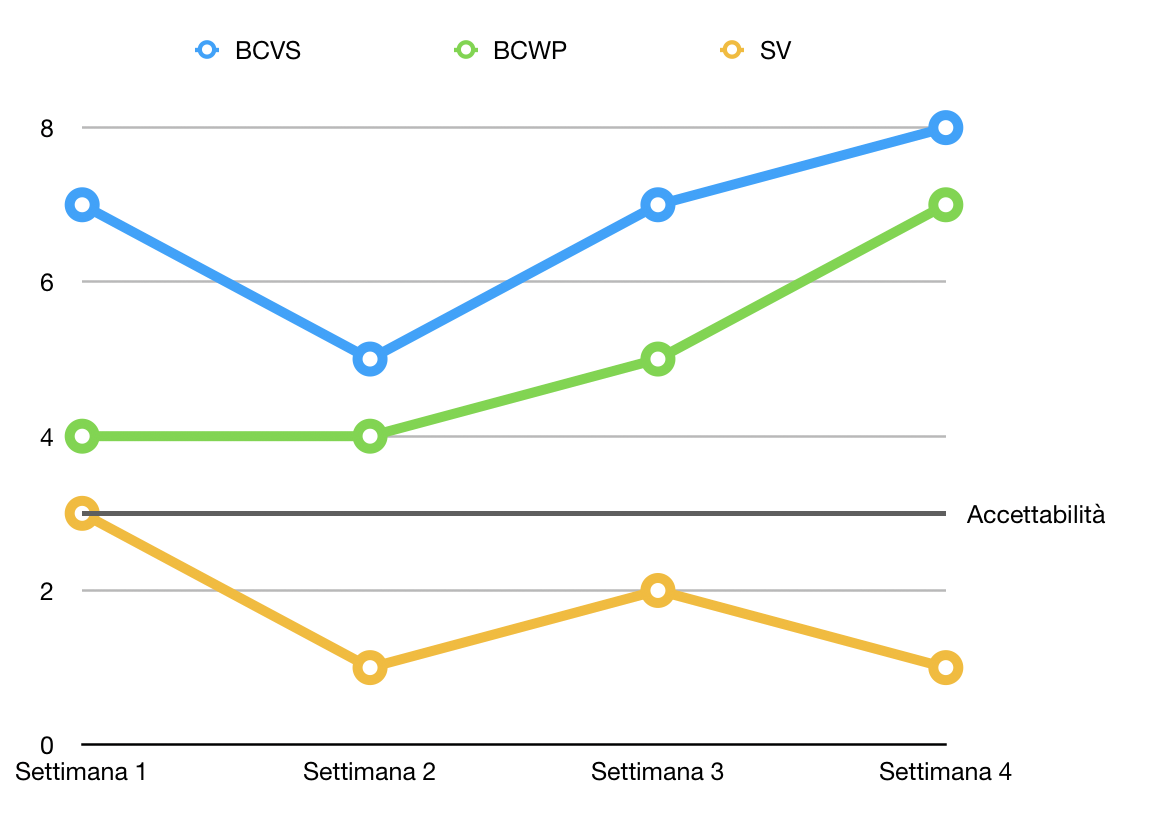
\includegraphics[scale=0.5]{./images/grafici_RA/MTPC01.png} 
		\caption{RA: MTPC01}
	\end{center}
\end{figure}

\paragraph{PR02: Gestione dei Costi}
\subparagraph{MTPC02: Budget Variance}  \-\\

\begin{figure}[H]
	\begin{center}
		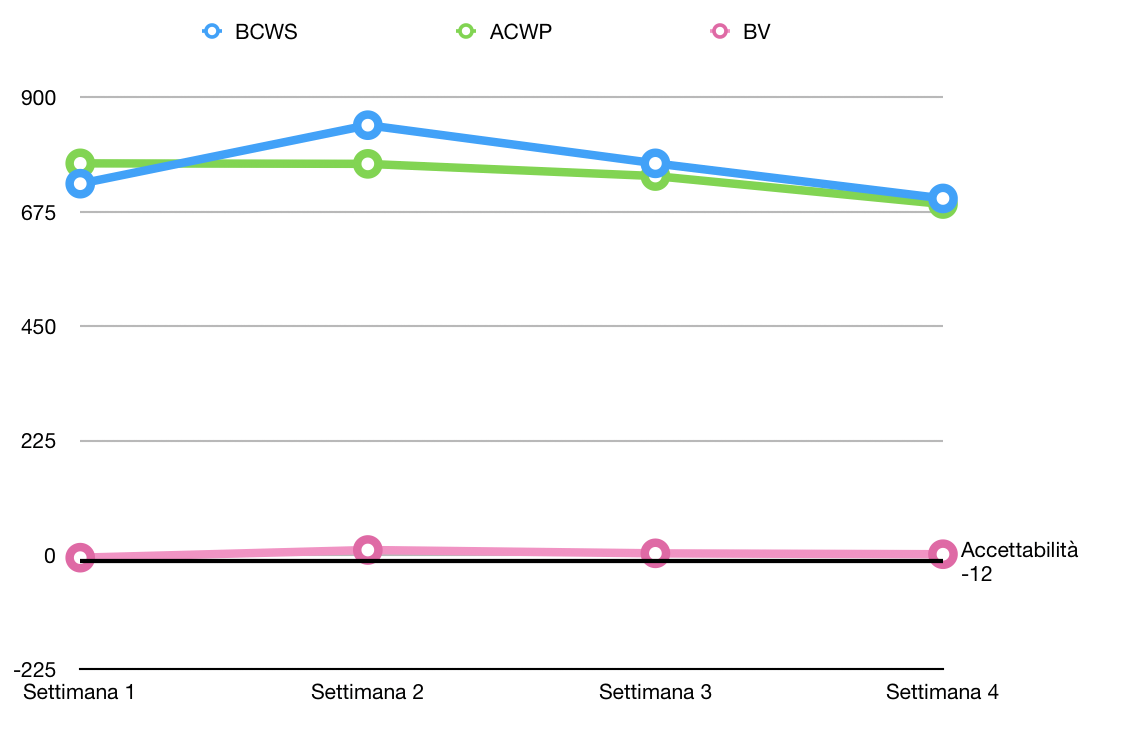
\includegraphics[scale=0.5]{./images/grafici_RA/MTPC02.png} 
		\caption{RA: MTPC02}
	\end{center}
\end{figure}

\subparagraph{MTPC03: Estimated at Completion}  \-\\

\begin{figure}[H]
	\begin{center}
		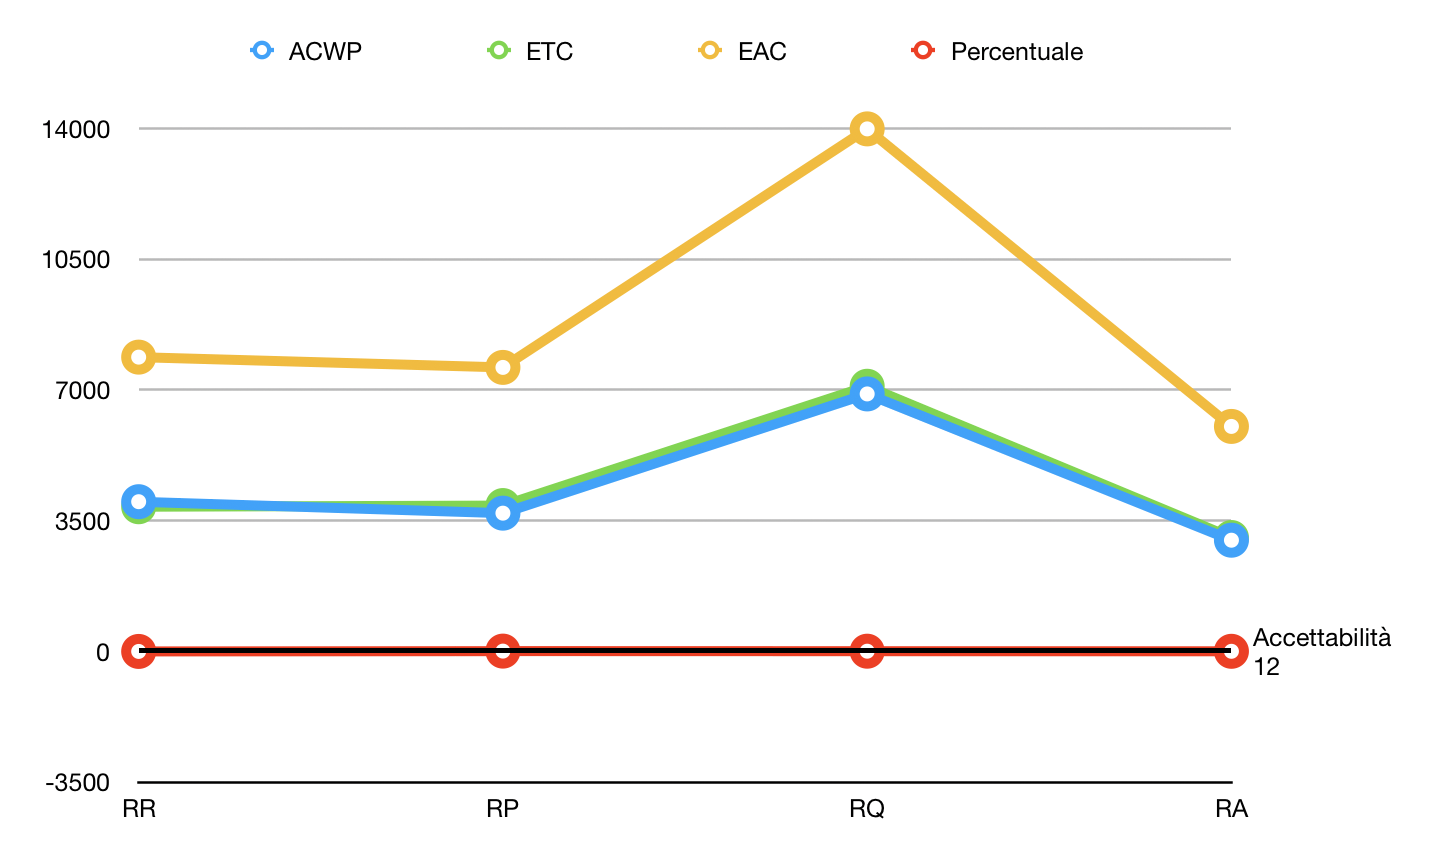
\includegraphics[scale=0.5]{./images/grafici_RA/MTPC03.png} 
		\caption{RA: MTPC03}
	\end{center}
\end{figure}

\paragraph{PR03: Verifica del Software}

\subparagraph{MTPC04 - MTPC05 - MTPC06 - MTCP07 - MTPC08}  \-\\

\begin{figure}[H]
	\begin{center}
		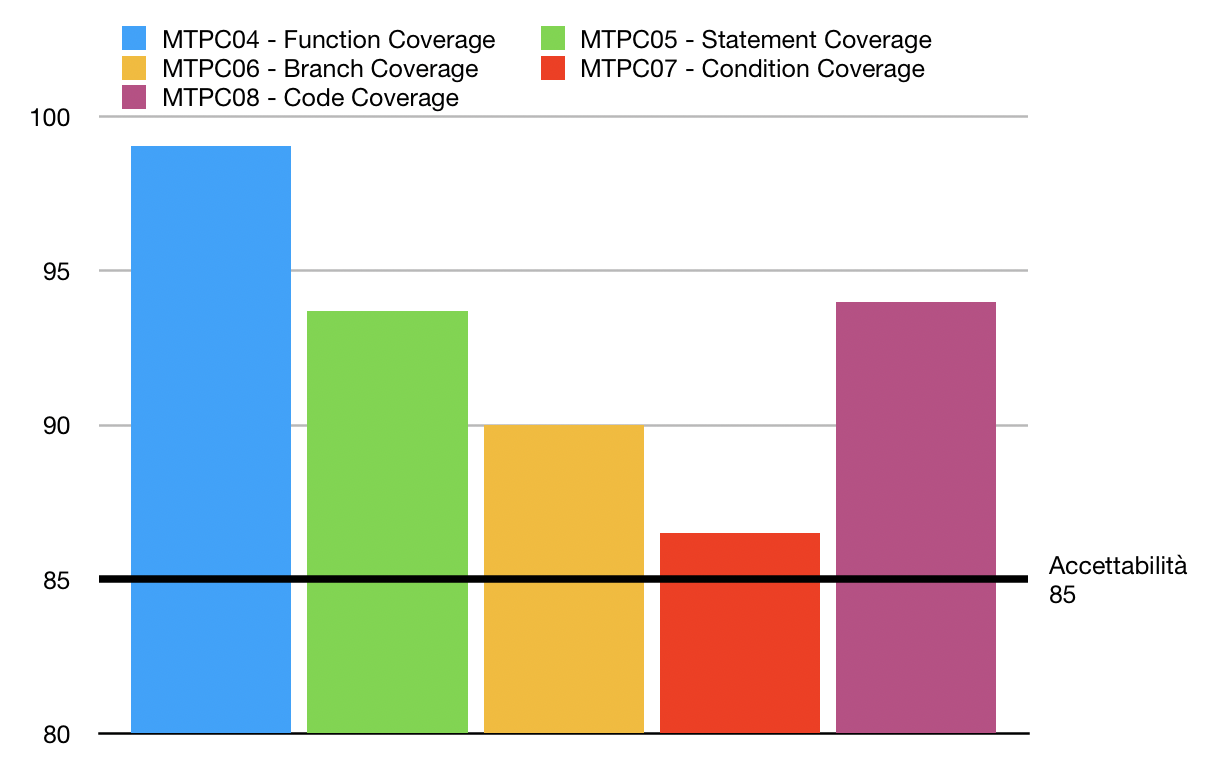
\includegraphics[scale=0.5]{./images/grafici_RA/PR03.png} 
		\caption{RA: MTPC04 - MTPC05 - MTPC06 - MTCP07 - MTPC08}
	\end{center}
\end{figure}

\paragraph{PR04: Gestione dei Rischi}
\subparagraph{MTPC09: Rischi non Preventivati} \-\\

\begin{figure}[H]
	\begin{center}
		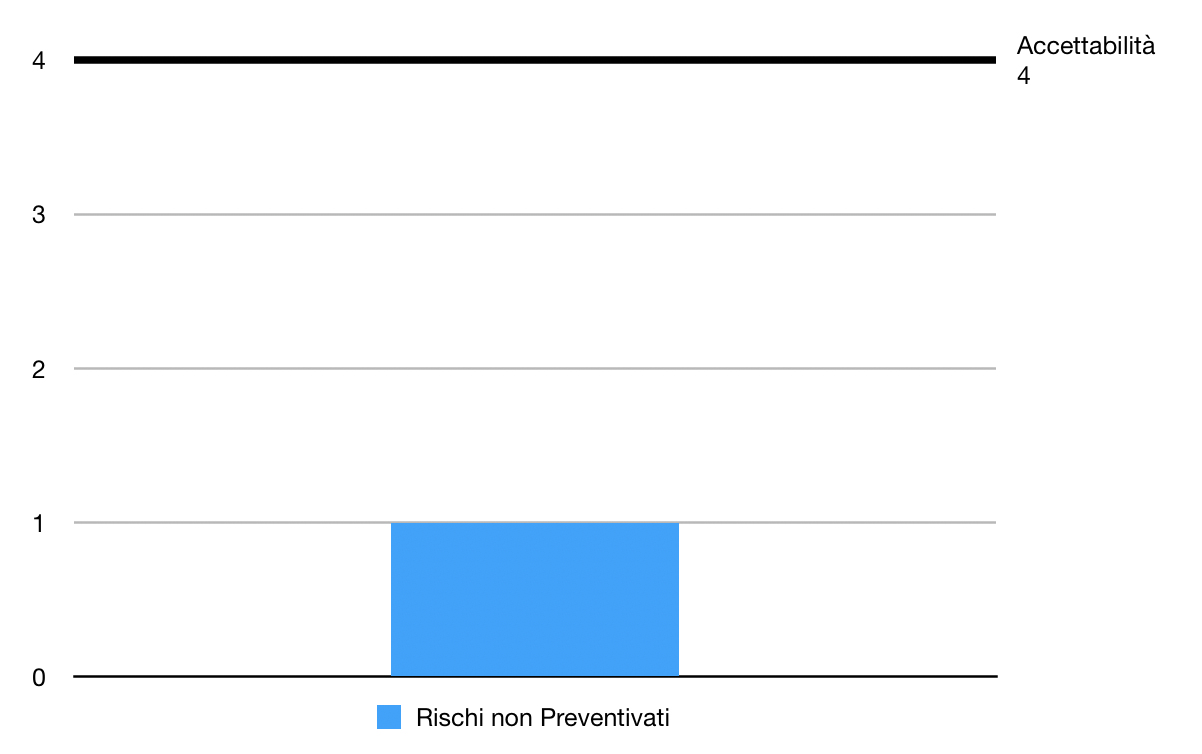
\includegraphics[scale=0.5]{./images/grafici_RA/MTPC09.png} 
		\caption{RA: MTPC09}
	\end{center}
\end{figure}

\paragraph{PR05: Gestione dei Test}
\subparagraph{MTTS10 - MTTS11 - MTTS12 - MTTS15 - MTTS16} \-\\

\begin{figure}[H]
	\begin{center}
		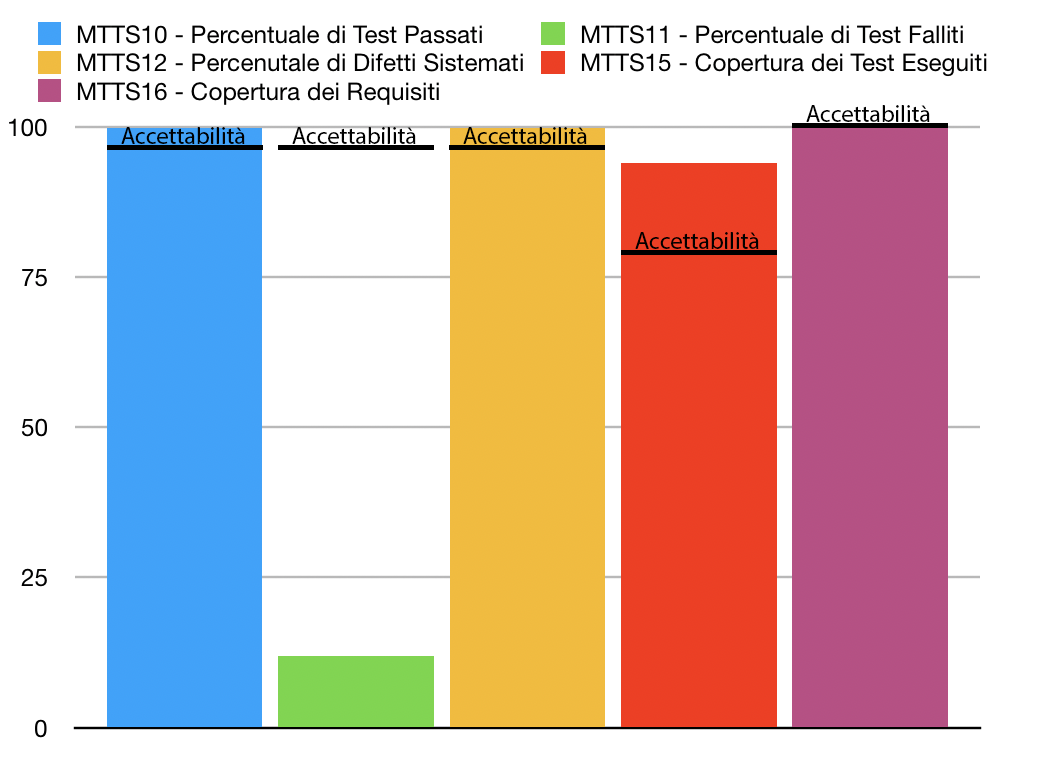
\includegraphics[scale=0.5]{./images/grafici_RA/PR05_percentuali.png} 
		\caption{RA: MTTS10 - MTTS11 - MTTS12 - MTTS15 - MTTS16}
	\end{center}
\end{figure}

\subparagraph{MTTS13: Tempo Medio di Risoluzione degli Errori} \-\\

\begin{figure}[H]
	\begin{center}
		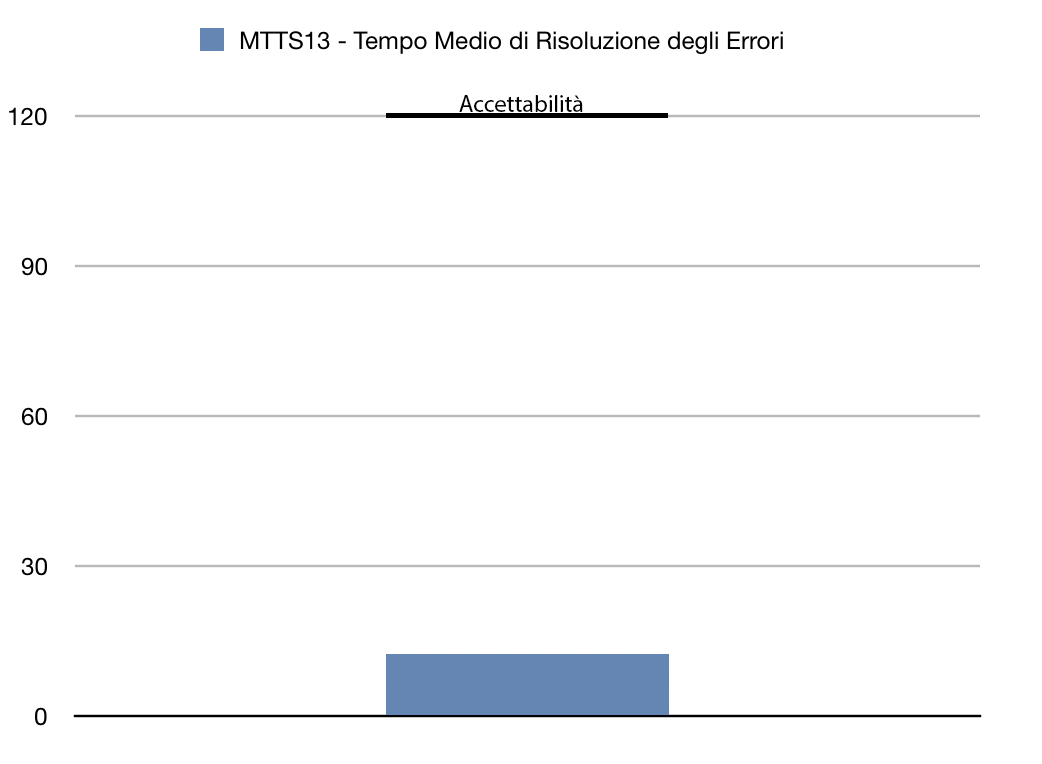
\includegraphics[scale=0.5]{./images/grafici_RA/PR05_temprisoluzioneerrori.png} 
		\caption{RA: MTTS13}
	\end{center}
\end{figure}

\subparagraph{MTTS14: Numero Medio di Bug Trovati per Test} \-\\

\begin{figure}[H]
	\begin{center}
		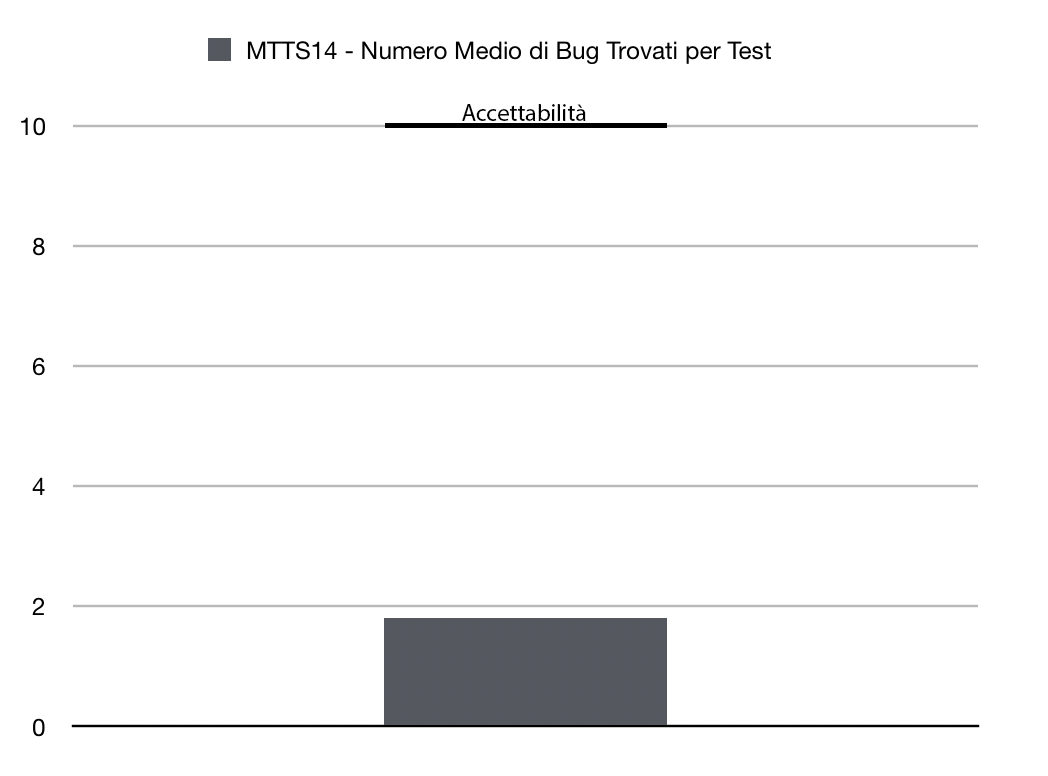
\includegraphics[scale=0.5]{./images/grafici_RA/PR05errorimedi.png} 
		\caption{RA: MTTS14}
	\end{center}
\end{figure}

\paragraph{PR06: Versionamento e Build}

\subparagraph{MTPC17: Media Commit per Settimana} \-\\

\begin{figure}[H]
	\begin{center}
		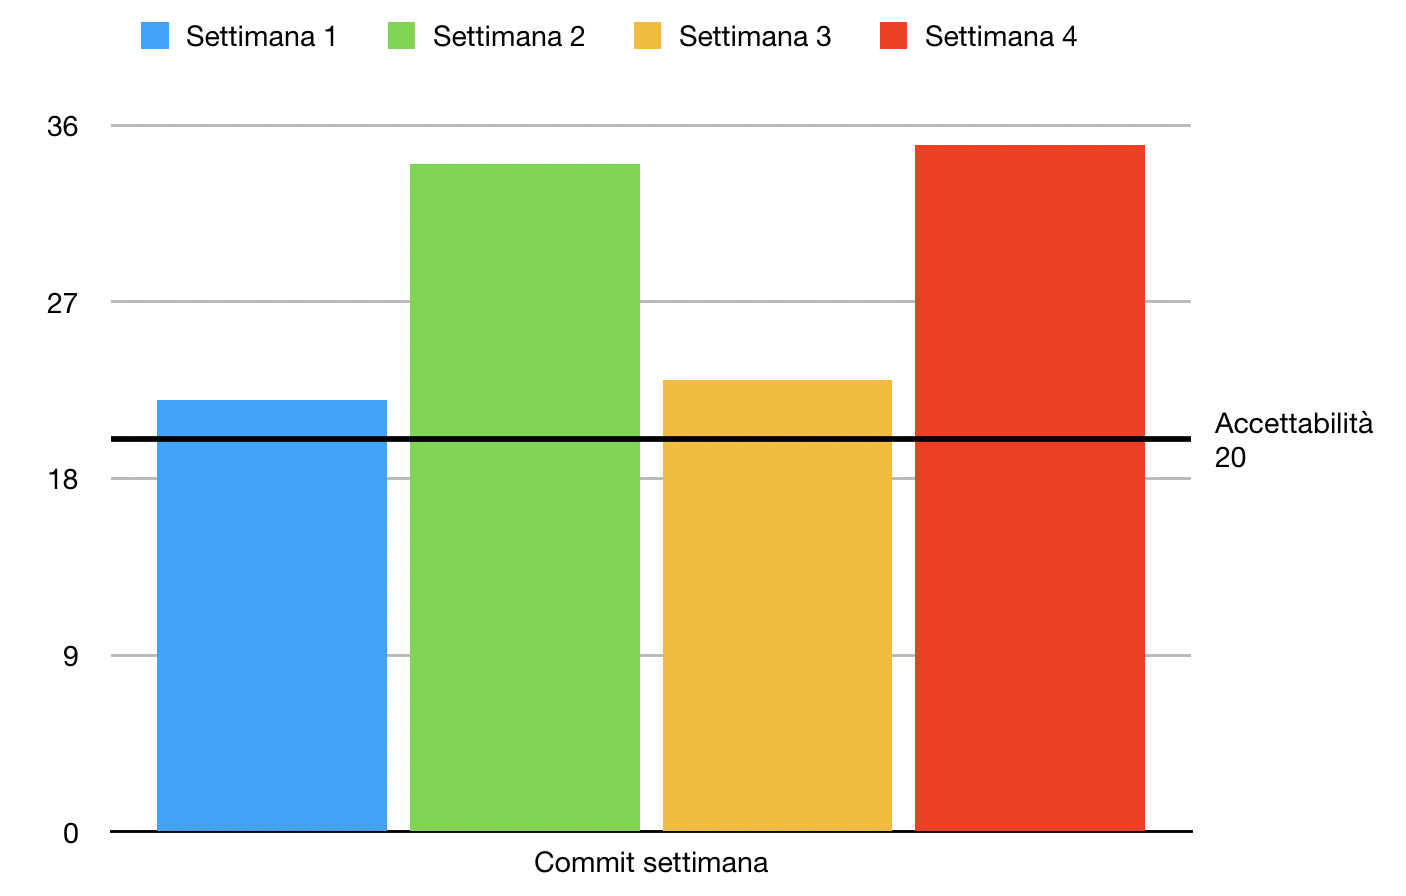
\includegraphics[scale=0.5]{./images/grafici_RA/MTPC17.png} 
		\caption{RA: MTPC17}
	\end{center}
\end{figure}

\subparagraph{MTPC18: Percentuali Build Superate } \-\\

\begin{longtable}{|C{.15\textwidth}|C{.24\textwidth}|C{.24\textwidth}|}
	\hline
	\rowcolor{bluelogo}\textbf{\textcolor{white}{Ottimalità}} & \textbf{\textcolor{white}{Accettabilità}} & \textbf{\textcolor{white}{Valore Misurato}} \\
	\hline \hline
	\endfirsthead
	$\geq 80$\% & $\geq 65$\% & 86.7\% \\
	\hline
	\caption{MTPC18 - Percentuale Build Superate}
\end{longtable}

\begin{figure}[H]
	\begin{center}
		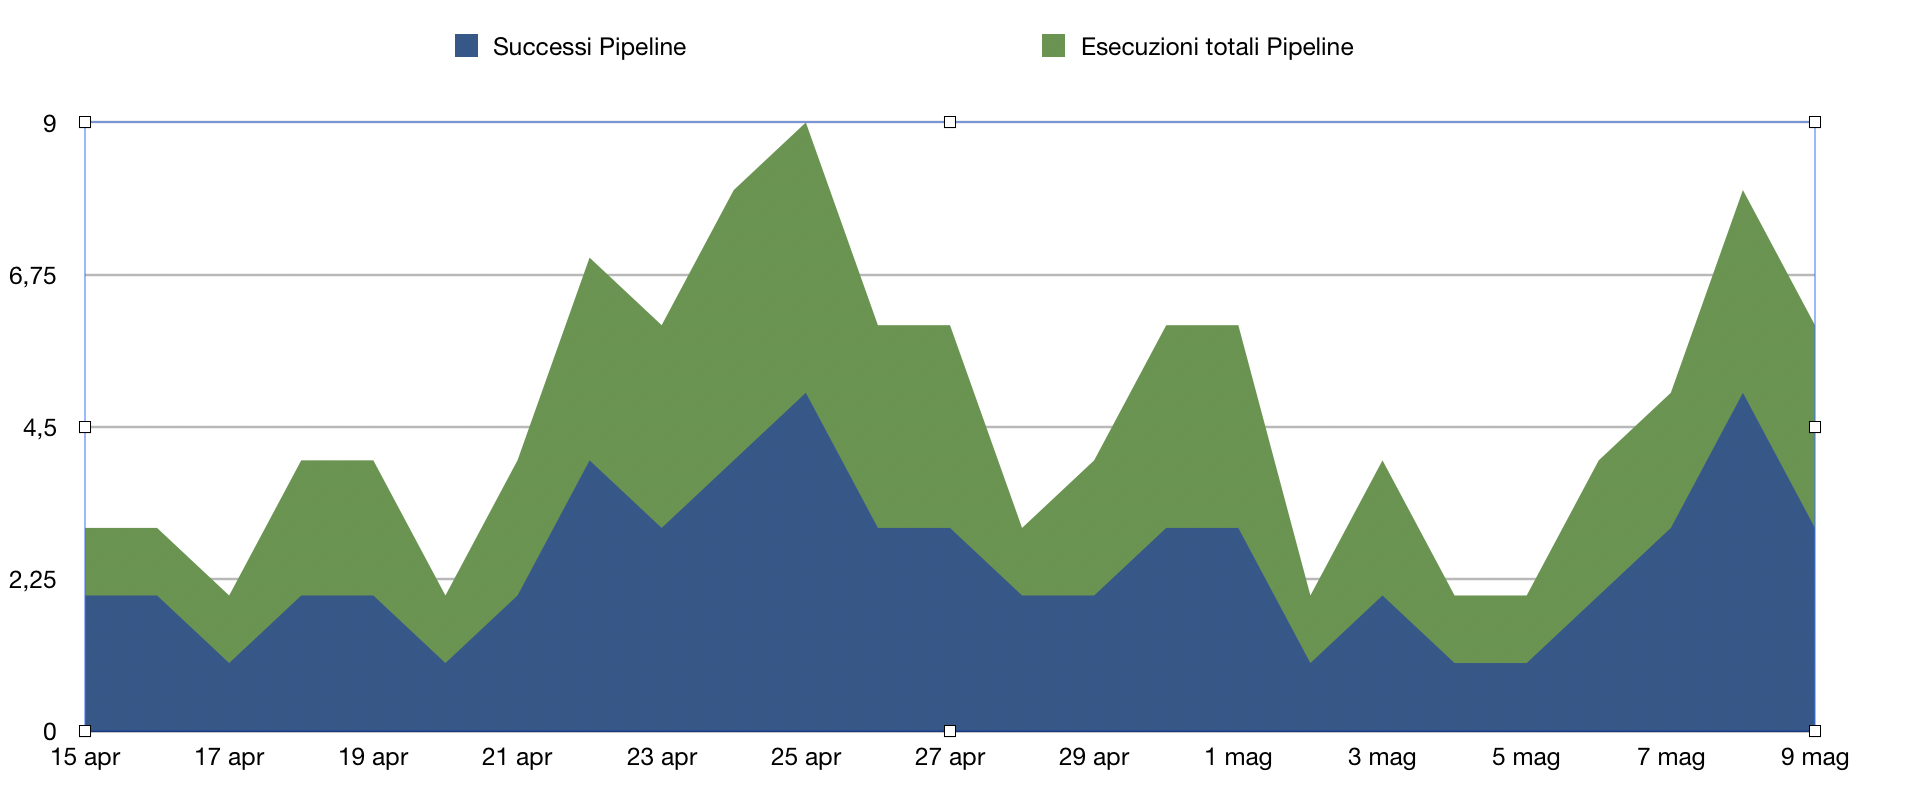
\includegraphics[scale=0.4]{./images/grafici_RA/MTPC18.png} 
		\caption{RA: MTPC18}
	\end{center}
\end{figure}

\paragraph{Comprensione}

\subparagraph{MTPDD19: Indice di Gulpease} \-\\

\begin{figure}[H]
	\begin{center}
		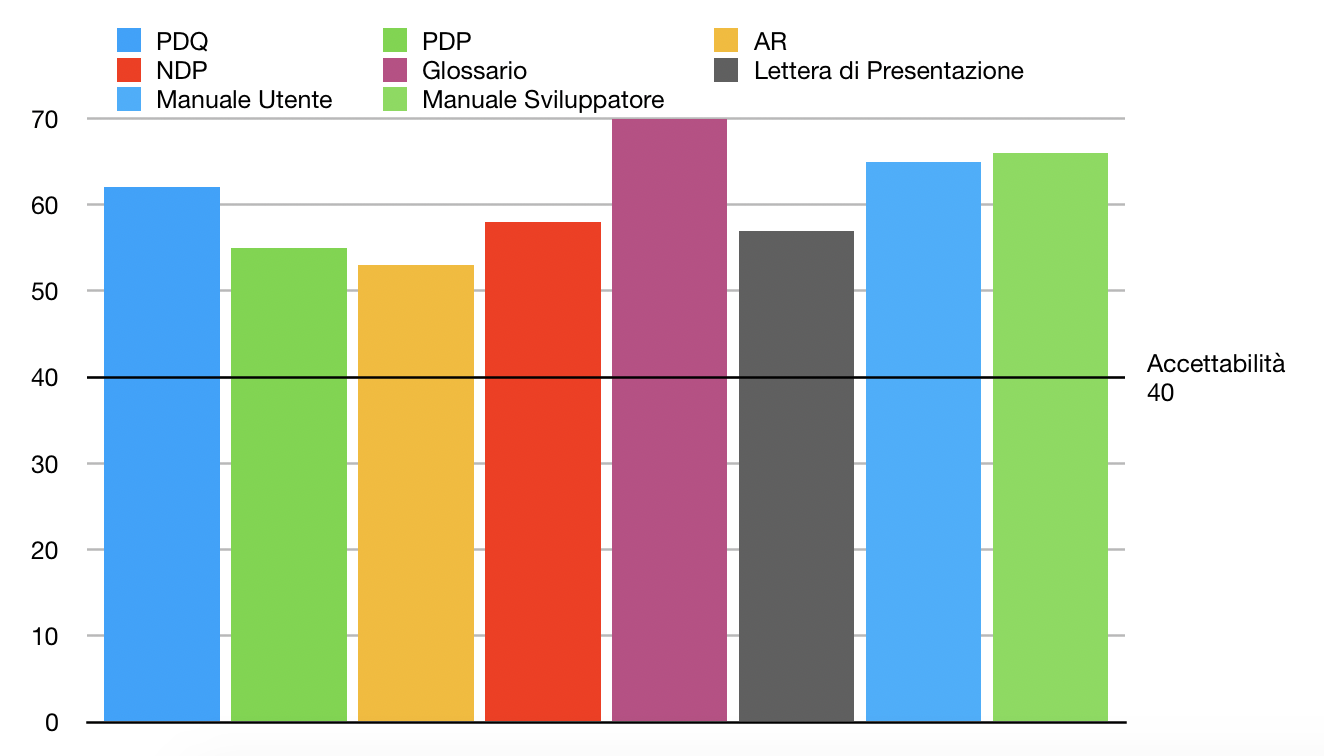
\includegraphics[scale=0.5]{./images/grafici_RA/MTPDD19.png} 
		\caption{RA: MTPDD19 - Documentazione}
	\end{center}
\end{figure}

\begin{figure}[H]
	\begin{center}
		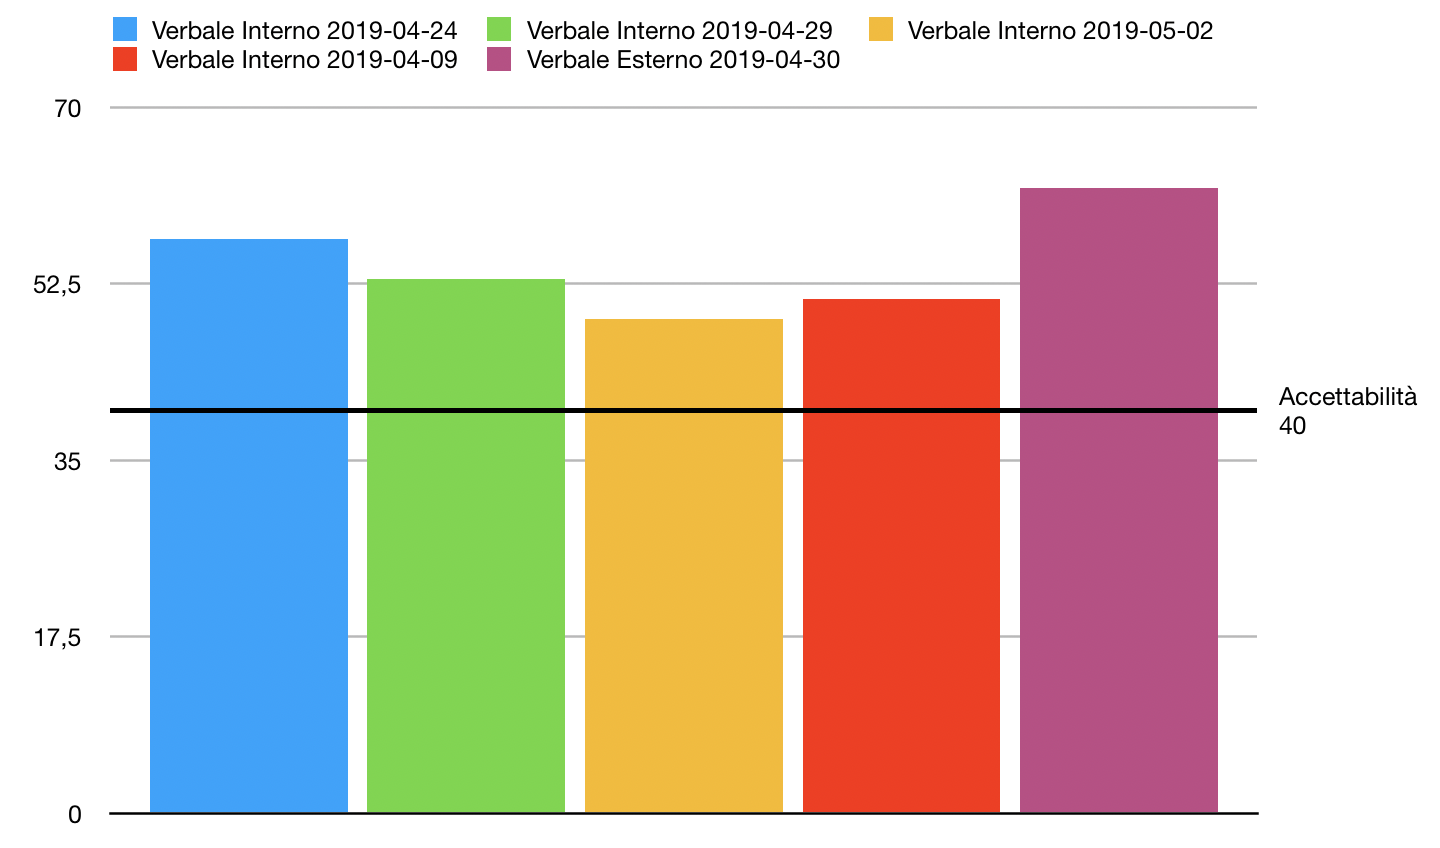
\includegraphics[scale=0.5]{./images/grafici_RA/MTPDD19-Verbali.png} 
		\caption{RA: MTPDD19 - Verbali}
	\end{center}
\end{figure}

\subparagraph{MTPDD20: Correttezza Ortografica} \-\\

\begin{figure}[H]
	\begin{center}
		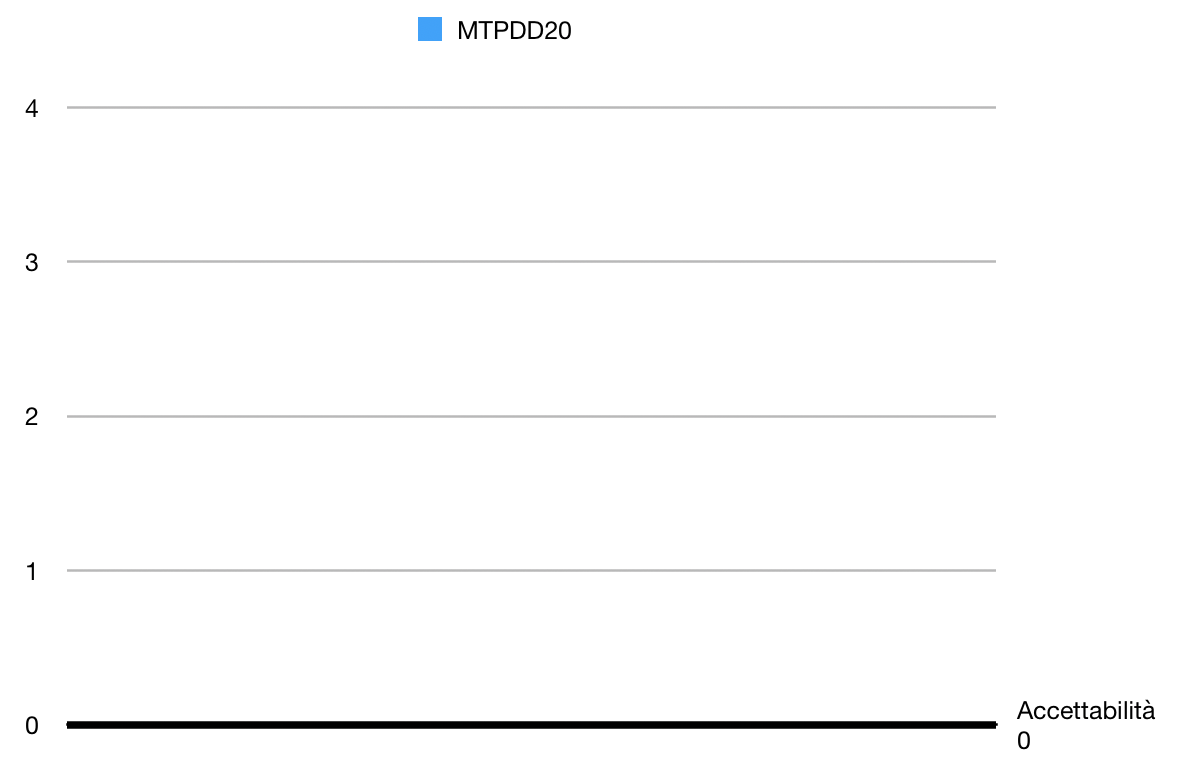
\includegraphics[scale=0.5]{./images/grafici_RA/MTPDD20.png} 
		\caption{RA: MTPDD20}
	\end{center}
\end{figure}

\paragraph{Funzionalità}

\subparagraph{MTPDS21 - MTPDS22 - MTPDS23} \-\\

\begin{figure}[H]
	\begin{center}
		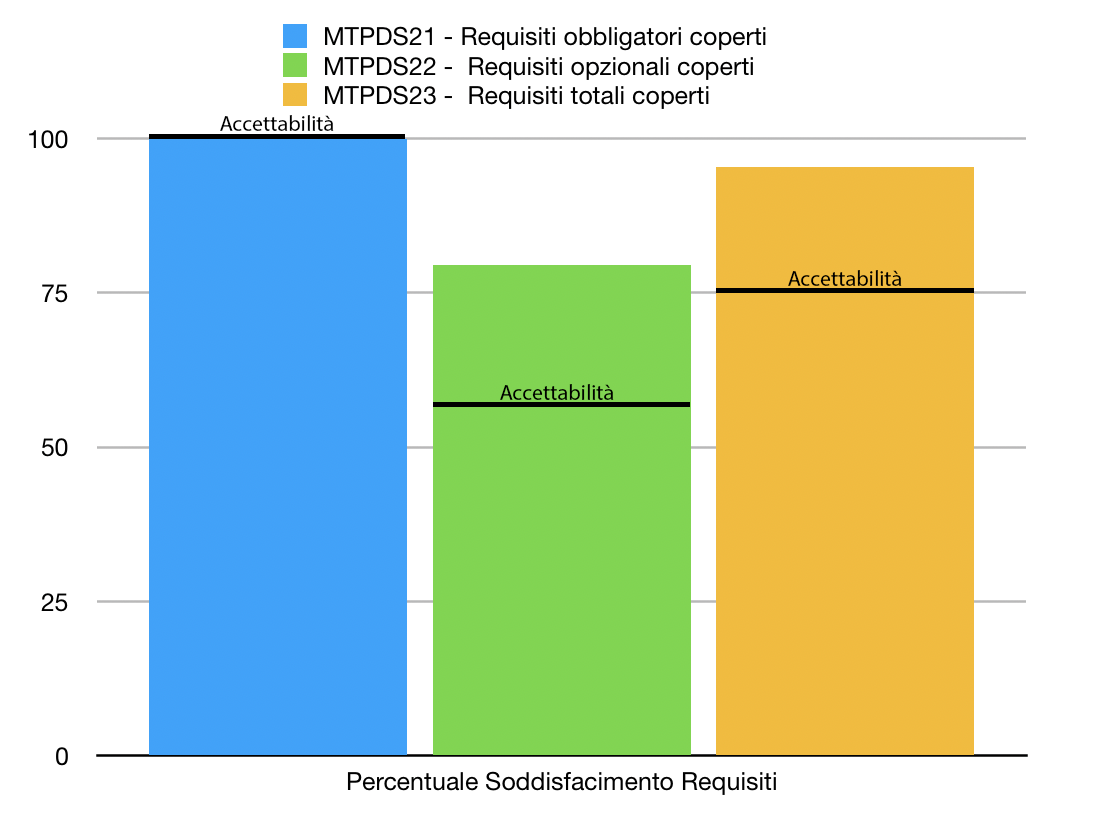
\includegraphics[scale=0.5]{./images/grafici_RA/Funzionalita.png} 
		\caption{RA: MTPDS21 - MTPDS22 - MTPDS2}
	\end{center}
\end{figure}

\paragraph{Affidabilità}

\subparagraph{MTPDS24 - MTPDS25} \-\\

\begin{figure}[H]
	\begin{center}
		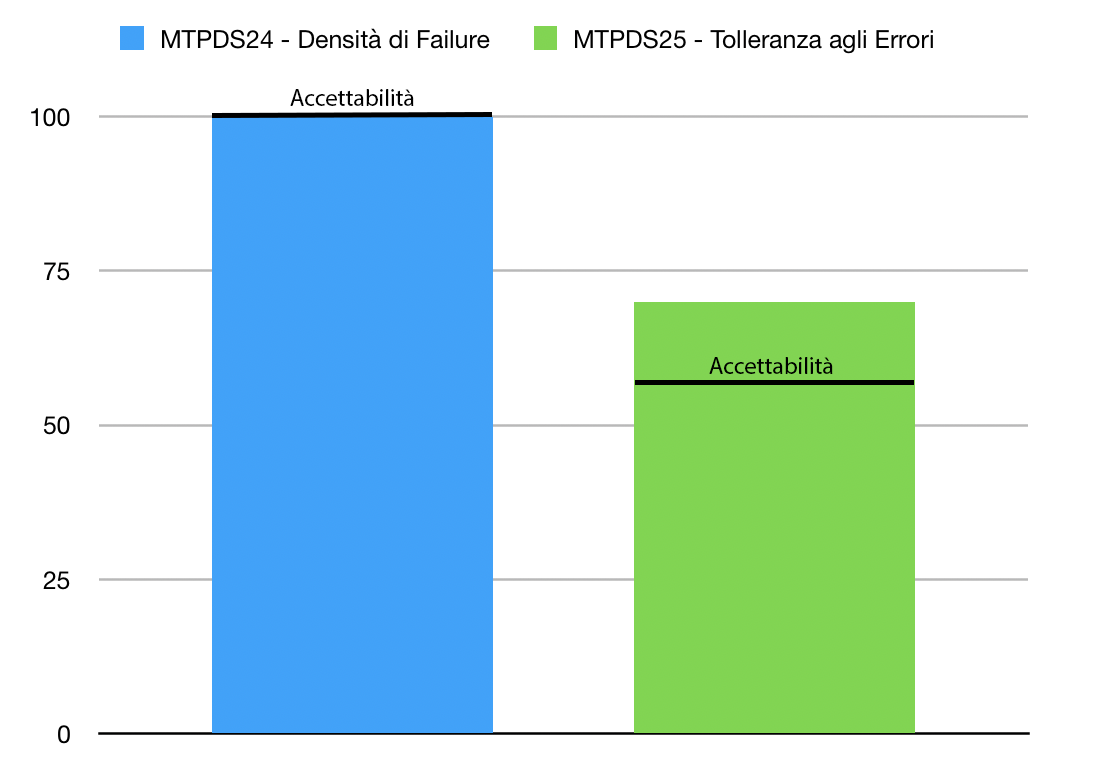
\includegraphics[scale=0.5]{./images/grafici_RA/Affidabilita.png} 
		\caption{RA: MTPDS24 - MTPDS25}
	\end{center}
\end{figure}

\paragraph{Efficienza}

\subparagraph{MTPDS26 - MTPDS27} \-\\

\begin{figure}[H]
	\begin{center}
		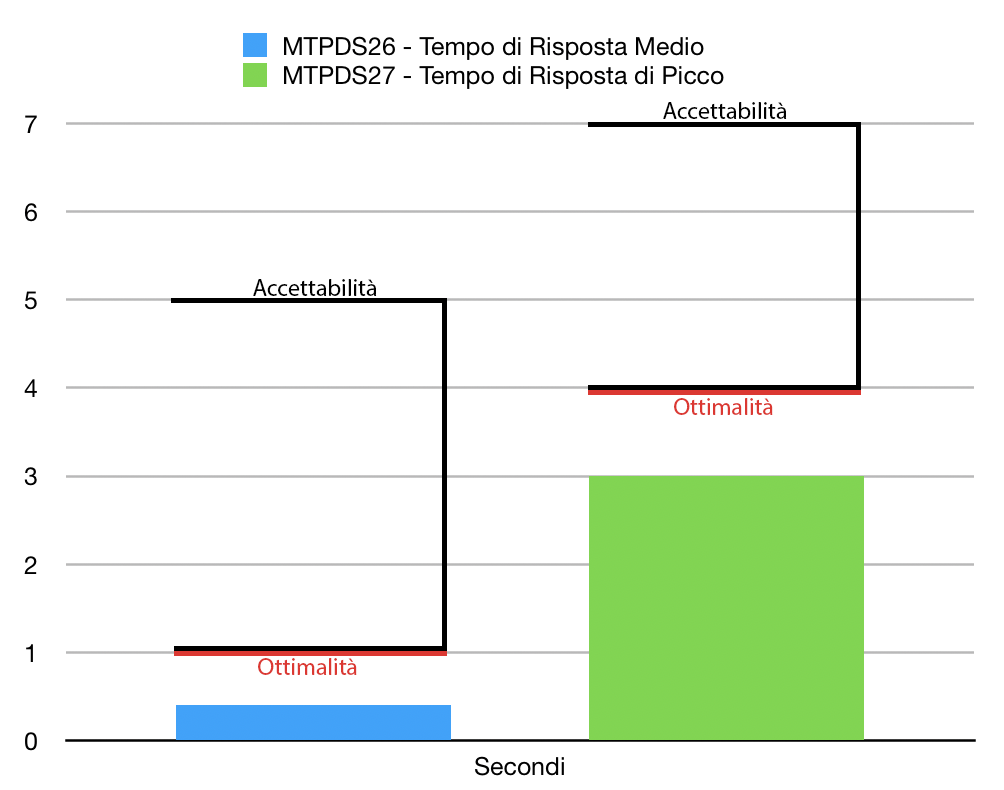
\includegraphics[scale=0.5]{./images/grafici_RA/Efficienza.png} 
		\caption{RA: MTPDS26 - MTPDS27}
	\end{center}
\end{figure}

\paragraph{Usabilità}

\subparagraph{MTPDS28 - MTPDS29} \-\\

\begin{figure}[H]
	\begin{center}
		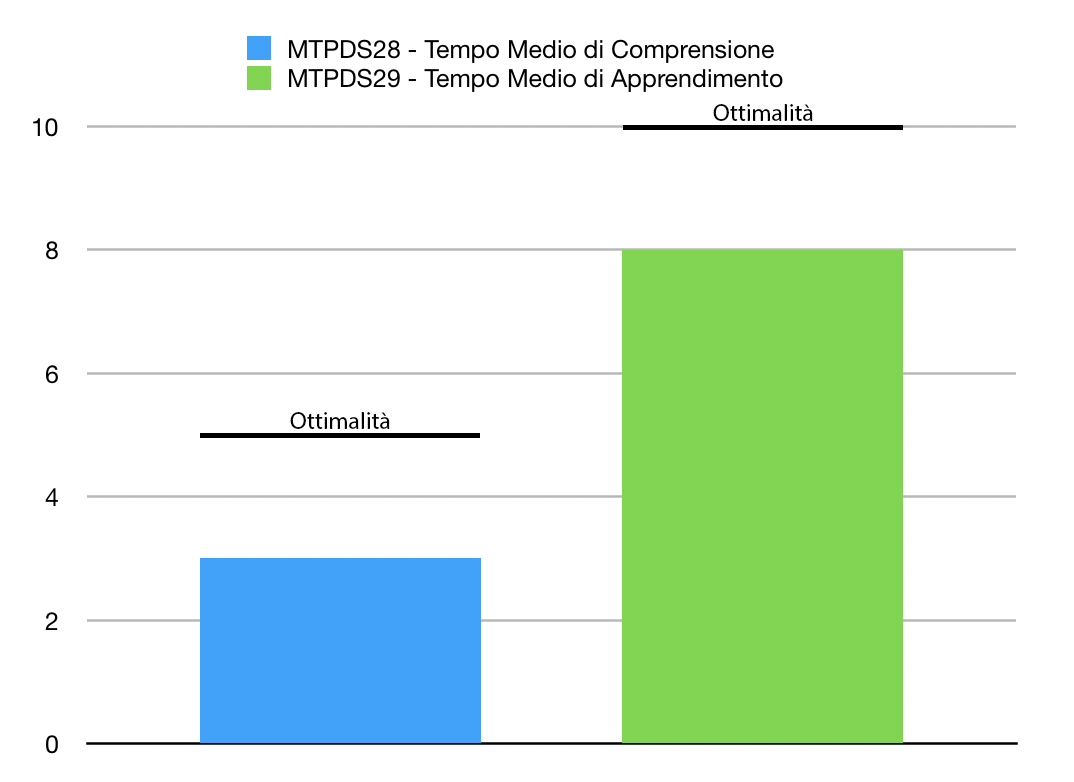
\includegraphics[scale=0.5]{./images/grafici_RA/Usabilita.png} 
		\caption{RA: MTPDS28 - MTPDS29}
	\end{center}
\end{figure}

\paragraph{Manutenibilità} 

\subparagraph{MTPDS30: Percentuale Commenti/Codice} \-\\

\begin{figure}[H]
	\begin{center}
		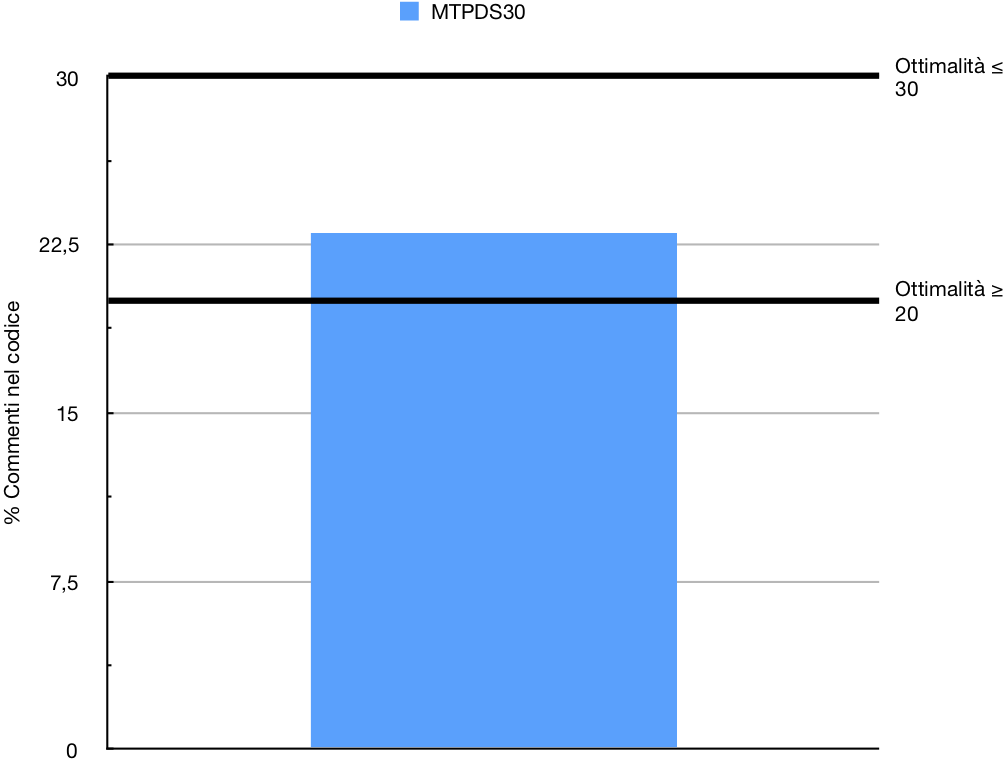
\includegraphics[scale=0.5]{./images/grafici_RA/MTPDS30.png} 
		\caption{RA: MTPDS30}
	\end{center}
\end{figure}